\chapter{Introduction}

The market for wireless loudspeakers has been growing considerably the last few years. According to Consumer Technology Association (CTA) the revenue of wireless loudspeakers has been growing 69\% between 2013 and 2014 \cite{sou:CTA}. The high growth is partly due to the increasing usage of smartphones and music streaming services, such as Spotify. As a result it is now more desirable for some users to wirelessly connect the smartphone to an audio system through for instance Bluetooth. By doing so, the user can use the smartphone as remote controller. 

Wireless loudspeakers are primarily active loudspeakers and are usually small. The size of the loudspeaker unit is therefore limited, and as a result the loudspeaker may not play very loud and the performance of the loudspeaker in the bass region is limited. To compensate for the lack of bass the user may want to boost the bass in order to achieve a more rich sound. However because of the limited size, increasing the bass can potentially lead to sound distortions caused by clipping or enclosure vibrations.


%Active loudspeakers are loudspeakers with an integrated amplifier used to drive the loudspeakers, since the signal from the smartphone do not have enough power.  


%Small loudspeakers grows in popularity
% Wireless loudspeakers are popular
% Smartphones and music streaming services are becoming popular
% Because of their wireless connectivity people desires audio solution were they can connect to their audio system through i.e. Wifi or Bluetooth. 
% 

% More people nowadays desires small loudspeaker, because of their portability and price.
% The market for small loudspeakers are therefore growing
% However even though the market is growing the performance of the small loudspeaker is still not necerssarily good.
% Because of their small sizes, there are limitations on 



\begin{figure}[H]
\centering
\tikzsetnextfilename{signal}
% This file was created by matlab2tikz.
%
%The latest updates can be retrieved from
%  http://www.mathworks.com/matlabcentral/fileexchange/22022-matlab2tikz-matlab2tikz
%where you can also make suggestions and rate matlab2tikz.
%
\definecolor{mycolor1}{rgb}{0.00000,0.44700,0.74100}%
\definecolor{mycolor2}{rgb}{0.85000,0.32500,0.09800}%
%
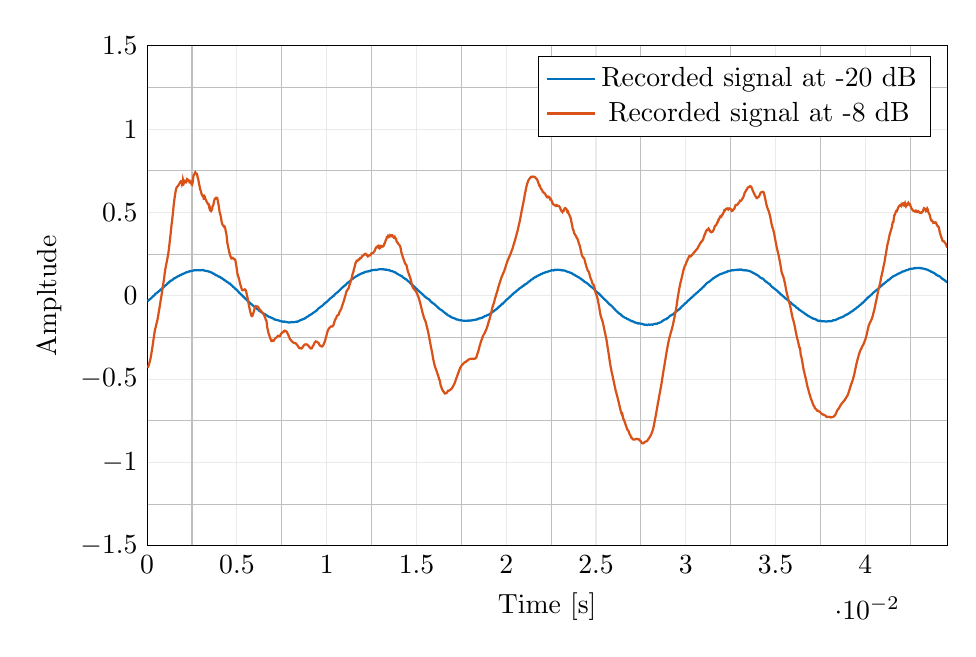
\begin{tikzpicture}

\begin{axis}[%
width=4in,
height=2.5in,
    grid = both,
    minor tick num=1,
    every major grid/.style={opacity=0.3},
    major tick length=0pt,
    minor tick length=0pt,
scale only axis,
xmin=0,
xmax=0.0445578231292517,
xlabel={Time [s]},
ymin=-1.5,
ymax=1.5,
ylabel={Ampltude},
axis background/.style={fill=white}
]
\addplot [color=mycolor1,solid,thick]
  table[row sep=crcr]{%
2.26757369614512e-05	-0.0328369140625\\
4.53514739229025e-05	-0.02972412109375\\
6.80272108843537e-05	-0.027435302734375\\
9.0702947845805e-05	-0.024932861328125\\
0.000113378684807256	-0.023895263671875\\
0.000136054421768707	-0.02191162109375\\
0.000158730158730159	-0.01983642578125\\
0.00018140589569161	-0.018402099609375\\
0.000204081632653061	-0.01605224609375\\
0.000226757369614512	-0.014068603515625\\
0.000249433106575964	-0.011749267578125\\
0.000272108843537415	-0.009124755859375\\
0.000294784580498866	-0.006683349609375\\
0.000317460317460317	-0.00439453125\\
0.000340136054421769	-0.001434326171875\\
0.00036281179138322	0.000579833984375\\
0.000385487528344671	0.001953125\\
0.000408163265306122	0.003631591796875\\
0.000430839002267574	0.007354736328125\\
0.000453514739229025	0.0113525390625\\
0.000476190476190476	0.013397216796875\\
0.000498866213151927	0.01416015625\\
0.000521541950113379	0.0147705078125\\
0.00054421768707483	0.0172119140625\\
0.000566893424036281	0.020050048828125\\
0.000589569160997732	0.021759033203125\\
0.000612244897959184	0.0238037109375\\
0.000634920634920635	0.026397705078125\\
0.000657596371882086	0.027740478515625\\
0.000680272108843537	0.02886962890625\\
0.000702947845804989	0.031829833984375\\
0.00072562358276644	0.03570556640625\\
0.000748299319727891	0.0372314453125\\
0.000770975056689342	0.038848876953125\\
0.000793650793650794	0.041229248046875\\
0.000816326530612245	0.0435791015625\\
0.000839002267573696	0.0457763671875\\
0.000861678004535147	0.047821044921875\\
0.000884353741496599	0.050567626953125\\
0.00090702947845805	0.05145263671875\\
0.000929705215419501	0.052490234375\\
0.000952380952380952	0.0550537109375\\
0.000975056689342404	0.05914306640625\\
0.000997732426303855	0.0614013671875\\
0.00102040816326531	0.062103271484375\\
0.00104308390022676	0.06439208984375\\
0.00106575963718821	0.066558837890625\\
0.00108843537414966	0.068572998046875\\
0.00111111111111111	0.0709228515625\\
0.00113378684807256	0.074066162109375\\
0.00115646258503401	0.076202392578125\\
0.00117913832199546	0.077545166015625\\
0.00120181405895692	0.079559326171875\\
0.00122448979591837	0.0819091796875\\
0.00124716553287982	0.0850830078125\\
0.00126984126984127	0.08746337890625\\
0.00129251700680272	0.08843994140625\\
0.00131519274376417	0.09027099609375\\
0.00133786848072562	0.09173583984375\\
0.00136054421768707	0.0921630859375\\
0.00138321995464853	0.09375\\
0.00140589569160998	0.095672607421875\\
0.00142857142857143	0.097320556640625\\
0.00145124716553288	0.099090576171875\\
0.00147392290249433	0.101531982421875\\
0.00149659863945578	0.104339599609375\\
0.00151927437641723	0.10528564453125\\
0.00154195011337868	0.106475830078125\\
0.00156462585034014	0.107421875\\
0.00158730158730159	0.108673095703125\\
0.00160997732426304	0.1104736328125\\
0.00163265306122449	0.1121826171875\\
0.00165532879818594	0.113677978515625\\
0.00167800453514739	0.11480712890625\\
0.00170068027210884	0.115875244140625\\
0.00172335600907029	0.116790771484375\\
0.00174603174603175	0.118560791015625\\
0.0017687074829932	0.119781494140625\\
0.00179138321995465	0.120635986328125\\
0.0018140589569161	0.122283935546875\\
0.00183673469387755	0.123809814453125\\
0.001859410430839	0.125030517578125\\
0.00188208616780045	0.124969482421875\\
0.0019047619047619	0.1268310546875\\
0.00192743764172336	0.128265380859375\\
0.00195011337868481	0.129302978515625\\
0.00197278911564626	0.130584716796875\\
0.00199546485260771	0.1318359375\\
0.00201814058956916	0.132537841796875\\
0.00204081632653061	0.13311767578125\\
0.00206349206349206	0.134429931640625\\
0.00208616780045351	0.13665771484375\\
0.00210884353741497	0.13739013671875\\
0.00213151927437642	0.137847900390625\\
0.00215419501133787	0.13946533203125\\
0.00217687074829932	0.1407470703125\\
0.00219954648526077	0.14117431640625\\
0.00222222222222222	0.140960693359375\\
0.00224489795918367	0.14215087890625\\
0.00226757369614512	0.143341064453125\\
0.00229024943310658	0.14422607421875\\
0.00231292517006803	0.144805908203125\\
0.00233560090702948	0.146392822265625\\
0.00235827664399093	0.14703369140625\\
0.00238095238095238	0.14642333984375\\
0.00240362811791383	0.14752197265625\\
0.00242630385487528	0.148284912109375\\
0.00244897959183673	0.148406982421875\\
0.00247165532879819	0.149078369140625\\
0.00249433106575964	0.149139404296875\\
0.00251700680272109	0.149993896484375\\
0.00253968253968254	0.151153564453125\\
0.00256235827664399	0.15118408203125\\
0.00258503401360544	0.151702880859375\\
0.00260770975056689	0.153106689453125\\
0.00263038548752834	0.15399169921875\\
0.0026530612244898	0.1534423828125\\
0.00267573696145125	0.1531982421875\\
0.0026984126984127	0.153533935546875\\
0.00272108843537415	0.15338134765625\\
0.0027437641723356	0.153411865234375\\
0.00276643990929705	0.153961181640625\\
0.0027891156462585	0.154144287109375\\
0.00281179138321995	0.15386962890625\\
0.00283446712018141	0.153717041015625\\
0.00285714285714286	0.1539306640625\\
0.00287981859410431	0.153778076171875\\
0.00290249433106576	0.1533203125\\
0.00292517006802721	0.1531982421875\\
0.00294784580498866	0.153472900390625\\
0.00297052154195011	0.153350830078125\\
0.00299319727891156	0.15325927734375\\
0.00301587301587302	0.1533203125\\
0.00303854875283447	0.154144287109375\\
0.00306122448979592	0.15496826171875\\
0.00308390022675737	0.15557861328125\\
0.00310657596371882	0.1551513671875\\
0.00312925170068027	0.153656005859375\\
0.00315192743764172	0.15228271484375\\
0.00317460317460317	0.151397705078125\\
0.00319727891156463	0.151763916015625\\
0.00321995464852608	0.151275634765625\\
0.00324263038548753	0.149658203125\\
0.00326530612244898	0.1494140625\\
0.00328798185941043	0.149505615234375\\
0.00331065759637188	0.149322509765625\\
0.00333333333333333	0.14910888671875\\
0.00335600907029478	0.148101806640625\\
0.00337868480725624	0.14752197265625\\
0.00340136054421769	0.146392822265625\\
0.00342403628117914	0.1461181640625\\
0.00344671201814059	0.145416259765625\\
0.00346938775510204	0.143798828125\\
0.00349206349206349	0.14276123046875\\
0.00351473922902494	0.142303466796875\\
0.00353741496598639	0.1417236328125\\
0.00356009070294785	0.140625\\
0.0035827664399093	0.13922119140625\\
0.00360544217687075	0.1378173828125\\
0.0036281179138322	0.1368408203125\\
0.00365079365079365	0.1356201171875\\
0.0036734693877551	0.133758544921875\\
0.00369614512471655	0.132568359375\\
0.003718820861678	0.132232666015625\\
0.00374149659863946	0.130584716796875\\
0.00376417233560091	0.1282958984375\\
0.00378684807256236	0.12701416015625\\
0.00380952380952381	0.12591552734375\\
0.00383219954648526	0.123687744140625\\
0.00385487528344671	0.1226806640625\\
0.00387755102040816	0.122528076171875\\
0.00390022675736961	0.121734619140625\\
0.00392290249433107	0.118927001953125\\
0.00394557823129252	0.11669921875\\
0.00396825396825397	0.1163330078125\\
0.00399092970521542	0.116241455078125\\
0.00401360544217687	0.1156005859375\\
0.00403628117913832	0.11358642578125\\
0.00405895691609977	0.1124267578125\\
0.00408163265306122	0.1104736328125\\
0.00410430839002268	0.10821533203125\\
0.00412698412698413	0.1068115234375\\
0.00414965986394558	0.106536865234375\\
0.00417233560090703	0.1048583984375\\
0.00419501133786848	0.101898193359375\\
0.00421768707482993	0.100555419921875\\
0.00424036281179138	0.099365234375\\
0.00426303854875283	0.097900390625\\
0.00428571428571429	0.095703125\\
0.00430839002267574	0.094207763671875\\
0.00433106575963719	0.093353271484375\\
0.00435374149659864	0.0906982421875\\
0.00437641723356009	0.08831787109375\\
0.00439909297052154	0.087249755859375\\
0.00442176870748299	0.085906982421875\\
0.00444444444444444	0.084075927734375\\
0.0044671201814059	0.081939697265625\\
0.00448979591836735	0.080902099609375\\
0.0045124716553288	0.079864501953125\\
0.00453514739229025	0.07708740234375\\
0.0045578231292517	0.074920654296875\\
0.00458049886621315	0.073486328125\\
0.0046031746031746	0.073577880859375\\
0.00462585034013605	0.071044921875\\
0.00464852607709751	0.06787109375\\
0.00467120181405896	0.065948486328125\\
0.00469387755102041	0.064178466796875\\
0.00471655328798186	0.06201171875\\
0.00473922902494331	0.0595703125\\
0.00476190476190476	0.057464599609375\\
0.00478458049886621	0.0543212890625\\
0.00480725623582766	0.05194091796875\\
0.00482993197278912	0.050537109375\\
0.00485260770975057	0.049224853515625\\
0.00487528344671202	0.046630859375\\
0.00489795918367347	0.04290771484375\\
0.00492063492063492	0.040374755859375\\
0.00494331065759637	0.03961181640625\\
0.00496598639455782	0.037689208984375\\
0.00498866213151927	0.03509521484375\\
0.00501133786848073	0.033721923828125\\
0.00503401360544218	0.03094482421875\\
0.00505668934240363	0.0269775390625\\
0.00507936507936508	0.024444580078125\\
0.00510204081632653	0.022491455078125\\
0.00512471655328798	0.01904296875\\
0.00514739229024943	0.015899658203125\\
0.00517006802721088	0.014678955078125\\
0.00519274376417234	0.01312255859375\\
0.00521541950113379	0.009857177734375\\
0.00523809523809524	0.007110595703125\\
0.00526077097505669	0.00543212890625\\
0.00528344671201814	0.003265380859375\\
0.00530612244897959	0.00048828125\\
0.00532879818594104	-0.001556396484375\\
0.00535147392290249	-0.00384521484375\\
0.00537414965986395	-0.006439208984375\\
0.0053968253968254	-0.009033203125\\
0.00541950113378685	-0.011688232421875\\
0.0054421768707483	-0.013916015625\\
0.00546485260770975	-0.01617431640625\\
0.0054875283446712	-0.018646240234375\\
0.00551020408163265	-0.021026611328125\\
0.0055328798185941	-0.022247314453125\\
0.00555555555555555	-0.02508544921875\\
0.00557823129251701	-0.0284423828125\\
0.00560090702947846	-0.03082275390625\\
0.00562358276643991	-0.0318603515625\\
0.00564625850340136	-0.033935546875\\
0.00566893424036281	-0.03662109375\\
0.00569160997732426	-0.039215087890625\\
0.00571428571428571	-0.0421142578125\\
0.00573696145124717	-0.043975830078125\\
0.00575963718820862	-0.046478271484375\\
0.00578231292517007	-0.048004150390625\\
0.00580498866213152	-0.04962158203125\\
0.00582766439909297	-0.052490234375\\
0.00585034013605442	-0.05419921875\\
0.00587301587301587	-0.056610107421875\\
0.00589569160997732	-0.059234619140625\\
0.00591836734693878	-0.061187744140625\\
0.00594104308390023	-0.06317138671875\\
0.00596371882086168	-0.064971923828125\\
0.00598639455782313	-0.06671142578125\\
0.00600907029478458	-0.06817626953125\\
0.00603174603174603	-0.069183349609375\\
0.00605442176870748	-0.071868896484375\\
0.00607709750566893	-0.074310302734375\\
0.00609977324263039	-0.07647705078125\\
0.00612244897959184	-0.07861328125\\
0.00614512471655329	-0.080596923828125\\
0.00616780045351474	-0.081634521484375\\
0.00619047619047619	-0.08306884765625\\
0.00621315192743764	-0.08538818359375\\
0.00623582766439909	-0.088958740234375\\
0.00625850340136054	-0.091156005859375\\
0.00628117913832199	-0.0921630859375\\
0.00630385487528345	-0.0936279296875\\
0.0063265306122449	-0.095733642578125\\
0.00634920634920635	-0.0966796875\\
0.0063718820861678	-0.098663330078125\\
0.00639455782312925	-0.100433349609375\\
0.0064172335600907	-0.10113525390625\\
0.00643990929705215	-0.102874755859375\\
0.00646258503401361	-0.10498046875\\
0.00648526077097506	-0.10638427734375\\
0.00650793650793651	-0.107666015625\\
0.00653061224489796	-0.109283447265625\\
0.00655328798185941	-0.110809326171875\\
0.00657596371882086	-0.111907958984375\\
0.00659863945578231	-0.11358642578125\\
0.00662131519274376	-0.115692138671875\\
0.00664399092970522	-0.117156982421875\\
0.00666666666666667	-0.118743896484375\\
0.00668934240362812	-0.119415283203125\\
0.00671201814058957	-0.1209716796875\\
0.00673469387755102	-0.123077392578125\\
0.00675736961451247	-0.1243896484375\\
0.00678004535147392	-0.126068115234375\\
0.00680272108843537	-0.127105712890625\\
0.00682539682539682	-0.127685546875\\
0.00684807256235828	-0.12799072265625\\
0.00687074829931973	-0.128814697265625\\
0.00689342403628118	-0.13043212890625\\
0.00691609977324263	-0.132568359375\\
0.00693877551020408	-0.133453369140625\\
0.00696145124716553	-0.133331298828125\\
0.00698412698412698	-0.13427734375\\
0.00700680272108843	-0.1356201171875\\
0.00702947845804989	-0.137054443359375\\
0.00705215419501134	-0.138763427734375\\
0.00707482993197279	-0.140838623046875\\
0.00709750566893424	-0.14208984375\\
0.00712018140589569	-0.14202880859375\\
0.00714285714285714	-0.142822265625\\
0.00716553287981859	-0.1439208984375\\
0.00718820861678005	-0.1448974609375\\
0.0072108843537415	-0.144805908203125\\
0.00723356009070295	-0.145263671875\\
0.0072562358276644	-0.145721435546875\\
0.00727891156462585	-0.1466064453125\\
0.0073015873015873	-0.147430419921875\\
0.00732426303854875	-0.14752197265625\\
0.0073469387755102	-0.148681640625\\
0.00736961451247166	-0.150543212890625\\
0.00739229024943311	-0.151031494140625\\
0.00741496598639456	-0.151031494140625\\
0.00743764172335601	-0.152435302734375\\
0.00746031746031746	-0.15252685546875\\
0.00748299319727891	-0.15283203125\\
0.00750566893424036	-0.153472900390625\\
0.00752834467120181	-0.154327392578125\\
0.00755102040816326	-0.154876708984375\\
0.00757369614512472	-0.15576171875\\
0.00759637188208617	-0.1556396484375\\
0.00761904761904762	-0.1539306640625\\
0.00764172335600907	-0.153656005859375\\
0.00766439909297052	-0.15484619140625\\
0.00768707482993197	-0.156005859375\\
0.00770975056689342	-0.156768798828125\\
0.00773242630385487	-0.157623291015625\\
0.00775510204081633	-0.15716552734375\\
0.00777777777777778	-0.1573486328125\\
0.00780045351473923	-0.1578369140625\\
0.00782312925170068	-0.15850830078125\\
0.00784580498866213	-0.15899658203125\\
0.00786848072562358	-0.1597900390625\\
0.00789115646258503	-0.16033935546875\\
0.00791383219954649	-0.16058349609375\\
0.00793650793650794	-0.160400390625\\
0.00795918367346939	-0.159149169921875\\
0.00798185941043084	-0.1583251953125\\
0.00800453514739229	-0.15863037109375\\
0.00802721088435374	-0.1585693359375\\
0.00804988662131519	-0.157562255859375\\
0.00807256235827664	-0.157196044921875\\
0.0080952380952381	-0.15771484375\\
0.00811791383219955	-0.15899658203125\\
0.008140589569161	-0.158905029296875\\
0.00816326530612245	-0.158111572265625\\
0.0081859410430839	-0.157684326171875\\
0.00820861678004535	-0.156585693359375\\
0.0082312925170068	-0.15679931640625\\
0.00825396825396825	-0.156280517578125\\
0.00827664399092971	-0.15594482421875\\
0.00829931972789116	-0.155059814453125\\
0.00832199546485261	-0.154815673828125\\
0.00834467120181406	-0.155792236328125\\
0.00836734693877551	-0.155517578125\\
0.00839002267573696	-0.154205322265625\\
0.00841269841269841	-0.15264892578125\\
0.00843537414965987	-0.151611328125\\
0.00845804988662132	-0.1507568359375\\
0.00848072562358277	-0.149505615234375\\
0.00850340136054422	-0.147491455078125\\
0.00852607709750567	-0.146728515625\\
0.00854875283446712	-0.1458740234375\\
0.00857142857142857	-0.14483642578125\\
0.00859410430839002	-0.14447021484375\\
0.00861678004535148	-0.143798828125\\
0.00863945578231293	-0.14178466796875\\
0.00866213151927438	-0.139739990234375\\
0.00868480725623583	-0.139617919921875\\
0.00870748299319728	-0.139923095703125\\
0.00873015873015873	-0.138702392578125\\
0.00875283446712018	-0.1373291015625\\
0.00877551020408163	-0.1361083984375\\
0.00879818594104308	-0.134552001953125\\
0.00882086167800454	-0.13323974609375\\
0.00884353741496599	-0.131500244140625\\
0.00886621315192744	-0.1295166015625\\
0.00888888888888889	-0.126678466796875\\
0.00891156462585034	-0.12518310546875\\
0.00893424036281179	-0.12493896484375\\
0.00895691609977324	-0.123809814453125\\
0.00897959183673469	-0.1221923828125\\
0.00900226757369615	-0.119842529296875\\
0.0090249433106576	-0.11712646484375\\
0.00904761904761905	-0.116302490234375\\
0.0090702947845805	-0.115997314453125\\
0.00909297052154195	-0.114349365234375\\
0.0091156462585034	-0.112060546875\\
0.00913832199546485	-0.110565185546875\\
0.0091609977324263	-0.108978271484375\\
0.00918367346938776	-0.107635498046875\\
0.00920634920634921	-0.10589599609375\\
0.00922902494331066	-0.10406494140625\\
0.00925170068027211	-0.10211181640625\\
0.00927437641723356	-0.100341796875\\
0.00929705215419501	-0.09912109375\\
0.00931972789115646	-0.09722900390625\\
0.00934240362811791	-0.095306396484375\\
0.00936507936507937	-0.094024658203125\\
0.00938775510204082	-0.09228515625\\
0.00941043083900227	-0.090118408203125\\
0.00943310657596372	-0.088226318359375\\
0.00945578231292517	-0.08599853515625\\
0.00947845804988662	-0.0836181640625\\
0.00950113378684807	-0.080535888671875\\
0.00952380952380952	-0.077392578125\\
0.00954648526077098	-0.0758056640625\\
0.00956916099773243	-0.07415771484375\\
0.00959183673469388	-0.0726318359375\\
0.00961451247165533	-0.07061767578125\\
0.00963718820861678	-0.068328857421875\\
0.00965986394557823	-0.0660400390625\\
0.00968253968253968	-0.064208984375\\
0.00970521541950113	-0.06304931640625\\
0.00972789115646258	-0.062164306640625\\
0.00975056689342404	-0.060089111328125\\
0.00977324263038549	-0.058074951171875\\
0.00979591836734694	-0.0557861328125\\
0.00981859410430839	-0.053192138671875\\
0.00984126984126984	-0.050323486328125\\
0.00986394557823129	-0.0474853515625\\
0.00988662131519275	-0.046356201171875\\
0.0099092970521542	-0.044464111328125\\
0.00993197278911565	-0.041748046875\\
0.0099546485260771	-0.039825439453125\\
0.00997732426303855	-0.0382080078125\\
0.01	-0.036590576171875\\
0.0100226757369615	-0.034942626953125\\
0.0100453514739229	-0.032318115234375\\
0.0100680272108844	-0.02935791015625\\
0.0100907029478458	-0.027374267578125\\
0.0101133786848073	-0.025238037109375\\
0.0101360544217687	-0.022552490234375\\
0.0101587301587302	-0.0198974609375\\
0.0101814058956916	-0.016815185546875\\
0.0102040816326531	-0.014434814453125\\
0.0102267573696145	-0.01318359375\\
0.010249433106576	-0.011383056640625\\
0.0102721088435374	-0.0098876953125\\
0.0102947845804989	-0.007965087890625\\
0.0103174603174603	-0.005126953125\\
0.0103401360544218	-0.0029296875\\
0.0103628117913832	-0.00213623046875\\
0.0103854875283447	-0.001007080078125\\
0.0104081632653061	0.00177001953125\\
0.0104308390022676	0.005462646484375\\
0.010453514739229	0.008270263671875\\
0.0104761904761905	0.01031494140625\\
0.0104988662131519	0.012908935546875\\
0.0105215419501134	0.015167236328125\\
0.0105442176870748	0.01617431640625\\
0.0105668934240363	0.018280029296875\\
0.0105895691609977	0.020843505859375\\
0.0106122448979592	0.022064208984375\\
0.0106349206349206	0.02398681640625\\
0.0106575963718821	0.026580810546875\\
0.0106802721088435	0.02972412109375\\
0.010702947845805	0.031494140625\\
0.0107256235827664	0.033843994140625\\
0.0107482993197279	0.036865234375\\
0.0107709750566893	0.0390625\\
0.0107936507936508	0.04156494140625\\
0.0108163265306122	0.04388427734375\\
0.0108390022675737	0.04669189453125\\
0.0108616780045351	0.0487060546875\\
0.0108843537414966	0.050323486328125\\
0.0109070294784581	0.052825927734375\\
0.0109297052154195	0.055419921875\\
0.010952380952381	0.0567626953125\\
0.0109750566893424	0.058563232421875\\
0.0109977324263039	0.061065673828125\\
0.0110204081632653	0.062530517578125\\
0.0110430839002268	0.06451416015625\\
0.0110657596371882	0.06707763671875\\
0.0110884353741497	0.06982421875\\
0.0111111111111111	0.072723388671875\\
0.0111337868480726	0.07489013671875\\
0.011156462585034	0.07708740234375\\
0.0111791383219955	0.079132080078125\\
0.0112018140589569	0.0809326171875\\
0.0112244897959184	0.0823974609375\\
0.0112471655328798	0.08416748046875\\
0.0112698412698413	0.08587646484375\\
0.0112925170068027	0.088043212890625\\
0.0113151927437642	0.089996337890625\\
0.0113378684807256	0.09228515625\\
0.0113605442176871	0.09503173828125\\
0.0113832199546485	0.0972900390625\\
0.01140589569161	0.09942626953125\\
0.0114285714285714	0.100433349609375\\
0.0114512471655329	0.101715087890625\\
0.0114739229024943	0.104583740234375\\
0.0114965986394558	0.10662841796875\\
0.0115192743764172	0.1083984375\\
0.0115419501133787	0.110198974609375\\
0.0115646258503401	0.11138916015625\\
0.0115873015873016	0.112884521484375\\
0.011609977324263	0.11480712890625\\
0.0116326530612245	0.116668701171875\\
0.0116553287981859	0.117950439453125\\
0.0116780045351474	0.1182861328125\\
0.0117006802721088	0.119232177734375\\
0.0117233560090703	0.121429443359375\\
0.0117460317460317	0.123809814453125\\
0.0117687074829932	0.124908447265625\\
0.0117913832199546	0.1265869140625\\
0.0118140589569161	0.127288818359375\\
0.0118367346938776	0.127593994140625\\
0.011859410430839	0.129119873046875\\
0.0118820861678005	0.131317138671875\\
0.0119047619047619	0.132476806640625\\
0.0119274376417234	0.1331787109375\\
0.0119501133786848	0.134002685546875\\
0.0119727891156463	0.135345458984375\\
0.0119954648526077	0.135345458984375\\
0.0120181405895692	0.1363525390625\\
0.0120408163265306	0.138214111328125\\
0.0120634920634921	0.138702392578125\\
0.0120861678004535	0.139923095703125\\
0.012108843537415	0.141754150390625\\
0.0121315192743764	0.14300537109375\\
0.0121541950113379	0.143402099609375\\
0.0121768707482993	0.144195556640625\\
0.0121995464852608	0.145050048828125\\
0.0122222222222222	0.145050048828125\\
0.0122448979591837	0.145599365234375\\
0.0122675736961451	0.146484375\\
0.0122902494331066	0.14593505859375\\
0.012312925170068	0.146270751953125\\
0.0123356009070295	0.14764404296875\\
0.0123582766439909	0.149139404296875\\
0.0123809523809524	0.149444580078125\\
0.0124036281179138	0.14910888671875\\
0.0124263038548753	0.149261474609375\\
0.0124489795918367	0.150970458984375\\
0.0124716553287982	0.152740478515625\\
0.0124943310657596	0.153289794921875\\
0.0125170068027211	0.15325927734375\\
0.0125396825396825	0.1531982421875\\
0.012562358276644	0.154052734375\\
0.0125850340136054	0.154571533203125\\
0.0126077097505669	0.15447998046875\\
0.0126303854875283	0.15460205078125\\
0.0126530612244898	0.1549072265625\\
0.0126757369614512	0.15496826171875\\
0.0126984126984127	0.155975341796875\\
0.0127210884353742	0.155975341796875\\
0.0127437641723356	0.15521240234375\\
0.0127664399092971	0.155029296875\\
0.0127891156462585	0.155853271484375\\
0.01281179138322	0.156158447265625\\
0.0128344671201814	0.1572265625\\
0.0128571428571429	0.157928466796875\\
0.0128798185941043	0.158477783203125\\
0.0129024943310658	0.158660888671875\\
0.0129251700680272	0.158905029296875\\
0.0129478458049887	0.158782958984375\\
0.0129705215419501	0.15899658203125\\
0.0129931972789116	0.15887451171875\\
0.013015873015873	0.158660888671875\\
0.0130385487528345	0.159088134765625\\
0.0130612244897959	0.159271240234375\\
0.0130839002267574	0.159332275390625\\
0.0131065759637188	0.1590576171875\\
0.0131292517006803	0.15960693359375\\
0.0131519274376417	0.16015625\\
0.0131746031746032	0.159393310546875\\
0.0131972789115646	0.157867431640625\\
0.0132199546485261	0.15838623046875\\
0.0132426303854875	0.158477783203125\\
0.013265306122449	0.156585693359375\\
0.0132879818594104	0.155853271484375\\
0.0133106575963719	0.156890869140625\\
0.0133333333333333	0.157440185546875\\
0.0133560090702948	0.156524658203125\\
0.0133786848072562	0.155364990234375\\
0.0134013605442177	0.15557861328125\\
0.0134240362811791	0.154815673828125\\
0.0134467120181406	0.153778076171875\\
0.013469387755102	0.15411376953125\\
0.0134920634920635	0.154815673828125\\
0.0135147392290249	0.152618408203125\\
0.0135374149659864	0.150787353515625\\
0.0135600907029478	0.149505615234375\\
0.0135827664399093	0.148529052734375\\
0.0136054421768707	0.148284912109375\\
0.0136281179138322	0.14788818359375\\
0.0136507936507937	0.14752197265625\\
0.0136734693877551	0.146575927734375\\
0.0136961451247166	0.14599609375\\
0.013718820861678	0.144866943359375\\
0.0137414965986395	0.142913818359375\\
0.0137641723356009	0.1414794921875\\
0.0137868480725624	0.141082763671875\\
0.0138095238095238	0.14105224609375\\
0.0138321995464853	0.139678955078125\\
0.0138548752834467	0.138092041015625\\
0.0138775510204082	0.13580322265625\\
0.0139002267573696	0.13458251953125\\
0.0139229024943311	0.13323974609375\\
0.0139455782312925	0.1309814453125\\
0.013968253968254	0.129638671875\\
0.0139909297052154	0.128204345703125\\
0.0140136054421769	0.127105712890625\\
0.0140362811791383	0.125885009765625\\
0.0140589569160998	0.12457275390625\\
0.0140816326530612	0.123077392578125\\
0.0141043083900227	0.12127685546875\\
0.0141269841269841	0.120208740234375\\
0.0141496598639456	0.119110107421875\\
0.014172335600907	0.1182861328125\\
0.0141950113378685	0.117095947265625\\
0.0142176870748299	0.114959716796875\\
0.0142403628117914	0.11138916015625\\
0.0142630385487528	0.10968017578125\\
0.0142857142857143	0.10858154296875\\
0.0143083900226757	0.107330322265625\\
0.0143310657596372	0.105316162109375\\
0.0143537414965986	0.103057861328125\\
0.0143764172335601	0.100738525390625\\
0.0143990929705215	0.099761962890625\\
0.014421768707483	0.09967041015625\\
0.0144444444444444	0.097747802734375\\
0.0144671201814059	0.094696044921875\\
0.0144897959183673	0.091888427734375\\
0.0145124716553288	0.089996337890625\\
0.0145351473922903	0.08746337890625\\
0.0145578231292517	0.086334228515625\\
0.0145804988662132	0.084869384765625\\
0.0146031746031746	0.083160400390625\\
0.0146258503401361	0.079742431640625\\
0.0146485260770975	0.076171875\\
0.014671201814059	0.0738525390625\\
0.0146938775510204	0.0712890625\\
0.0147165532879819	0.06915283203125\\
0.0147392290249433	0.067779541015625\\
0.0147619047619048	0.06646728515625\\
0.0147845804988662	0.063995361328125\\
0.0148072562358277	0.06103515625\\
0.0148299319727891	0.059326171875\\
0.0148526077097506	0.057525634765625\\
0.014875283446712	0.055328369140625\\
0.0148979591836735	0.052520751953125\\
0.0149206349206349	0.049957275390625\\
0.0149433106575964	0.0472412109375\\
0.0149659863945578	0.04473876953125\\
0.0149886621315193	0.04302978515625\\
0.0150113378684807	0.0411376953125\\
0.0150340136054422	0.038726806640625\\
0.0150566893424036	0.0352783203125\\
0.0150793650793651	0.0333251953125\\
0.0151020408163265	0.031463623046875\\
0.015124716553288	0.028900146484375\\
0.0151473922902494	0.026702880859375\\
0.0151700680272109	0.024627685546875\\
0.0151927437641723	0.022369384765625\\
0.0152154195011338	0.02020263671875\\
0.0152380952380952	0.018829345703125\\
0.0152607709750567	0.016754150390625\\
0.0152834467120181	0.01416015625\\
0.0153061224489796	0.01171875\\
0.015328798185941	0.009429931640625\\
0.0153514739229025	0.007781982421875\\
0.0153741496598639	0.005615234375\\
0.0153968253968254	0.0032958984375\\
0.0154195011337868	0.0009765625\\
0.0154421768707483	-0.00201416015625\\
0.0154648526077098	-0.004364013671875\\
0.0154875283446712	-0.0064697265625\\
0.0155102040816327	-0.00860595703125\\
0.0155328798185941	-0.009735107421875\\
0.0155555555555556	-0.011322021484375\\
0.015578231292517	-0.01348876953125\\
0.0156009070294785	-0.01568603515625\\
0.0156235827664399	-0.01666259765625\\
0.0156462585034014	-0.017852783203125\\
0.0156689342403628	-0.01934814453125\\
0.0156916099773243	-0.021240234375\\
0.0157142857142857	-0.023712158203125\\
0.0157369614512472	-0.026275634765625\\
0.0157596371882086	-0.0291748046875\\
0.0157823129251701	-0.0325927734375\\
0.0158049886621315	-0.035186767578125\\
0.015827664399093	-0.036285400390625\\
0.0158503401360544	-0.038238525390625\\
0.0158730158730159	-0.040802001953125\\
0.0158956916099773	-0.0426025390625\\
0.0159183673469388	-0.044769287109375\\
0.0159410430839002	-0.046173095703125\\
0.0159637188208617	-0.0474853515625\\
0.0159863945578231	-0.048858642578125\\
0.0160090702947846	-0.050628662109375\\
0.016031746031746	-0.05303955078125\\
0.0160544217687075	-0.05584716796875\\
0.0160770975056689	-0.057769775390625\\
0.0160997732426304	-0.06005859375\\
0.0161224489795918	-0.06268310546875\\
0.0161451247165533	-0.065032958984375\\
0.0161678004535147	-0.067047119140625\\
0.0161904761904762	-0.0689697265625\\
0.0162131519274376	-0.0711669921875\\
0.0162358276643991	-0.074493408203125\\
0.0162585034013605	-0.076171875\\
0.016281179138322	-0.07794189453125\\
0.0163038548752834	-0.080352783203125\\
0.0163265306122449	-0.08221435546875\\
0.0163492063492063	-0.082794189453125\\
0.0163718820861678	-0.084136962890625\\
0.0163945578231292	-0.086578369140625\\
0.0164172335600907	-0.087646484375\\
0.0164399092970522	-0.0894775390625\\
0.0164625850340136	-0.091949462890625\\
0.0164852607709751	-0.093994140625\\
0.0165079365079365	-0.0953369140625\\
0.016530612244898	-0.097625732421875\\
0.0165532879818594	-0.100006103515625\\
0.0165759637188209	-0.101837158203125\\
0.0165986394557823	-0.103424072265625\\
0.0166213151927438	-0.105255126953125\\
0.0166439909297052	-0.107421875\\
0.0166666666666667	-0.10906982421875\\
0.0166893424036281	-0.11077880859375\\
0.0167120181405896	-0.11328125\\
0.016734693877551	-0.11529541015625\\
0.0167573696145125	-0.116668701171875\\
0.0167800453514739	-0.117889404296875\\
0.0168027210884354	-0.119140625\\
0.0168253968253968	-0.119598388671875\\
0.0168480725623583	-0.120635986328125\\
0.0168707482993197	-0.123565673828125\\
0.0168934240362812	-0.125885009765625\\
0.0169160997732426	-0.126312255859375\\
0.0169387755102041	-0.127227783203125\\
0.0169614512471655	-0.12939453125\\
0.016984126984127	-0.130645751953125\\
0.0170068027210884	-0.1314697265625\\
0.0170294784580499	-0.132080078125\\
0.0170521541950113	-0.1326904296875\\
0.0170748299319728	-0.133270263671875\\
0.0170975056689342	-0.13458251953125\\
0.0171201814058957	-0.13555908203125\\
0.0171428571428571	-0.135986328125\\
0.0171655328798186	-0.137420654296875\\
0.01718820861678	-0.139556884765625\\
0.0172108843537415	-0.14117431640625\\
0.0172335600907029	-0.14178466796875\\
0.0172562358276644	-0.141876220703125\\
0.0172789115646259	-0.142120361328125\\
0.0173015873015873	-0.14288330078125\\
0.0173242630385488	-0.143218994140625\\
0.0173469387755102	-0.14434814453125\\
0.0173696145124717	-0.145751953125\\
0.0173922902494331	-0.14691162109375\\
0.0174149659863946	-0.147186279296875\\
0.017437641723356	-0.14617919921875\\
0.0174603174603175	-0.146331787109375\\
0.0174829931972789	-0.14691162109375\\
0.0175056689342404	-0.1473388671875\\
0.0175283446712018	-0.1478271484375\\
0.0175510204081633	-0.148406982421875\\
0.0175736961451247	-0.1488037109375\\
0.0175963718820862	-0.1490478515625\\
0.0176190476190476	-0.149383544921875\\
0.0176417233560091	-0.14990234375\\
0.0176643990929705	-0.14990234375\\
0.017687074829932	-0.149688720703125\\
0.0177097505668934	-0.14984130859375\\
0.0177324263038549	-0.149139404296875\\
0.0177551020408163	-0.15008544921875\\
0.0177777777777778	-0.1497802734375\\
0.0178004535147392	-0.149627685546875\\
0.0178231292517007	-0.149749755859375\\
0.0178458049886621	-0.149932861328125\\
0.0178684807256236	-0.149078369140625\\
0.017891156462585	-0.148193359375\\
0.0179138321995465	-0.148590087890625\\
0.0179365079365079	-0.149322509765625\\
0.0179591836734694	-0.1490478515625\\
0.0179818594104308	-0.148284912109375\\
0.0180045351473923	-0.14849853515625\\
0.0180272108843537	-0.148651123046875\\
0.0180498866213152	-0.1480712890625\\
0.0180725623582766	-0.146881103515625\\
0.0180952380952381	-0.147552490234375\\
0.0181179138321995	-0.147216796875\\
0.018140589569161	-0.145751953125\\
0.0181632653061224	-0.144561767578125\\
0.0181859410430839	-0.14483642578125\\
0.0182086167800454	-0.145233154296875\\
0.0182312925170068	-0.144500732421875\\
0.0182539682539683	-0.14404296875\\
0.0182766439909297	-0.144073486328125\\
0.0182993197278912	-0.14361572265625\\
0.0183219954648526	-0.14178466796875\\
0.0183446712018141	-0.14141845703125\\
0.0183673469387755	-0.1422119140625\\
0.018390022675737	-0.1402587890625\\
0.0184126984126984	-0.13824462890625\\
0.0184353741496599	-0.13775634765625\\
0.0184580498866213	-0.1373291015625\\
0.0184807256235828	-0.13616943359375\\
0.0185034013605442	-0.13531494140625\\
0.0185260770975057	-0.13568115234375\\
0.0185487528344671	-0.1353759765625\\
0.0185714285714286	-0.133941650390625\\
0.01859410430839	-0.13287353515625\\
0.0186167800453515	-0.13275146484375\\
0.0186394557823129	-0.132659912109375\\
0.0186621315192744	-0.130157470703125\\
0.0186848072562358	-0.12890625\\
0.0187074829931973	-0.1287841796875\\
0.0187301587301587	-0.12774658203125\\
0.0187528344671202	-0.125762939453125\\
0.0187755102040816	-0.123870849609375\\
0.0187981859410431	-0.122711181640625\\
0.0188208616780045	-0.12152099609375\\
0.018843537414966	-0.12139892578125\\
0.0188662131519274	-0.1207275390625\\
0.0188888888888889	-0.120147705078125\\
0.0189115646258503	-0.118194580078125\\
0.0189342403628118	-0.116729736328125\\
0.0189569160997732	-0.1153564453125\\
0.0189795918367347	-0.11468505859375\\
0.0190022675736961	-0.113922119140625\\
0.0190249433106576	-0.112640380859375\\
0.019047619047619	-0.111572265625\\
0.0190702947845805	-0.110443115234375\\
0.0190929705215419	-0.108673095703125\\
0.0191156462585034	-0.106109619140625\\
0.0191383219954649	-0.104705810546875\\
0.0191609977324263	-0.1031494140625\\
0.0191836734693878	-0.10125732421875\\
0.0192063492063492	-0.09954833984375\\
0.0192290249433107	-0.097503662109375\\
0.0192517006802721	-0.095367431640625\\
0.0192743764172336	-0.09442138671875\\
0.019297052154195	-0.092803955078125\\
0.0193197278911565	-0.091400146484375\\
0.0193424036281179	-0.08941650390625\\
0.0193650793650794	-0.086669921875\\
0.0193877551020408	-0.084747314453125\\
0.0194104308390023	-0.083038330078125\\
0.0194331065759637	-0.081756591796875\\
0.0194557823129252	-0.0799560546875\\
0.0194784580498866	-0.0780029296875\\
0.0195011337868481	-0.07513427734375\\
0.0195238095238095	-0.0731201171875\\
0.019546485260771	-0.071319580078125\\
0.0195691609977324	-0.069000244140625\\
0.0195918367346939	-0.0660400390625\\
0.0196145124716553	-0.06378173828125\\
0.0196371882086168	-0.062530517578125\\
0.0196598639455782	-0.061004638671875\\
0.0196825396825397	-0.058258056640625\\
0.0197052154195011	-0.05517578125\\
0.0197278911564626	-0.053131103515625\\
0.019750566893424	-0.050445556640625\\
0.0197732426303855	-0.04803466796875\\
0.0197959183673469	-0.04766845703125\\
0.0198185941043084	-0.046295166015625\\
0.0198412698412698	-0.04345703125\\
0.0198639455782313	-0.040313720703125\\
0.0198866213151927	-0.037811279296875\\
0.0199092970521542	-0.035552978515625\\
0.0199319727891156	-0.033050537109375\\
0.0199546485260771	-0.030731201171875\\
0.0199773242630385	-0.02783203125\\
0.02	-0.025482177734375\\
0.0200226757369615	-0.023101806640625\\
0.0200453514739229	-0.02105712890625\\
0.0200680272108844	-0.01971435546875\\
0.0200907029478458	-0.017822265625\\
0.0201133786848073	-0.015472412109375\\
0.0201360544217687	-0.012908935546875\\
0.0201587301587302	-0.010498046875\\
0.0201814058956916	-0.008636474609375\\
0.0202040816326531	-0.006072998046875\\
0.0202267573696145	-0.003173828125\\
0.020249433106576	-0.001953125\\
0.0202721088435374	0.0001220703125\\
0.0202947845804989	0.003082275390625\\
0.0203174603174603	0.00628662109375\\
0.0203401360544218	0.007843017578125\\
0.0203628117913832	0.009490966796875\\
0.0203854875283447	0.01275634765625\\
0.0204081632653061	0.014892578125\\
0.0204308390022676	0.016632080078125\\
0.020453514739229	0.018951416015625\\
0.0204761904761905	0.020233154296875\\
0.0204988662131519	0.0220947265625\\
0.0205215419501134	0.024078369140625\\
0.0205442176870748	0.026092529296875\\
0.0205668934240363	0.028778076171875\\
0.0205895691609977	0.0303955078125\\
0.0206122448979592	0.032073974609375\\
0.0206349206349206	0.034942626953125\\
0.0206575963718821	0.037384033203125\\
0.0206802721088435	0.0380859375\\
0.020702947845805	0.03985595703125\\
0.0207256235827664	0.042572021484375\\
0.0207482993197279	0.044830322265625\\
0.0207709750566893	0.04681396484375\\
0.0207936507936508	0.047882080078125\\
0.0208163265306122	0.049774169921875\\
0.0208390022675737	0.0513916015625\\
0.0208616780045351	0.0531005859375\\
0.0208843537414966	0.055084228515625\\
0.020907029478458	0.057342529296875\\
0.0209297052154195	0.05841064453125\\
0.020952380952381	0.05938720703125\\
0.0209750566893424	0.062042236328125\\
0.0209977324263039	0.064697265625\\
0.0210204081632653	0.0672607421875\\
0.0210430839002268	0.06768798828125\\
0.0210657596371882	0.0694580078125\\
0.0210884353741497	0.07049560546875\\
0.0211111111111111	0.07183837890625\\
0.0211337868480726	0.0733642578125\\
0.021156462585034	0.0748291015625\\
0.0211791383219955	0.077484130859375\\
0.0212018140589569	0.079345703125\\
0.0212244897959184	0.08148193359375\\
0.0212471655328798	0.084564208984375\\
0.0212698412698413	0.08587646484375\\
0.0212925170068027	0.0865478515625\\
0.0213151927437642	0.088470458984375\\
0.0213378684807256	0.090667724609375\\
0.0213605442176871	0.09368896484375\\
0.0213832199546485	0.095977783203125\\
0.02140589569161	0.097015380859375\\
0.0214285714285714	0.09808349609375\\
0.0214512471655329	0.100006103515625\\
0.0214739229024943	0.10205078125\\
0.0214965986394558	0.103271484375\\
0.0215192743764172	0.10540771484375\\
0.0215419501133787	0.10809326171875\\
0.0215646258503401	0.109222412109375\\
0.0215873015873016	0.1097412109375\\
0.021609977324263	0.1112060546875\\
0.0216326530612245	0.113494873046875\\
0.0216553287981859	0.114715576171875\\
0.0216780045351474	0.114593505859375\\
0.0217006802721088	0.11676025390625\\
0.0217233560090703	0.11883544921875\\
0.0217460317460317	0.119842529296875\\
0.0217687074829932	0.12091064453125\\
0.0217913832199546	0.1220703125\\
0.0218140589569161	0.124114990234375\\
0.0218367346938775	0.124237060546875\\
0.021859410430839	0.125\\
0.0218820861678005	0.1268310546875\\
0.0219047619047619	0.128692626953125\\
0.0219274376417234	0.130584716796875\\
0.0219501133786848	0.130706787109375\\
0.0219727891156463	0.130859375\\
0.0219954648526077	0.13232421875\\
0.0220181405895692	0.133819580078125\\
0.0220408163265306	0.135009765625\\
0.0220634920634921	0.136627197265625\\
0.0220861678004535	0.137298583984375\\
0.022108843537415	0.137969970703125\\
0.0221315192743764	0.13836669921875\\
0.0221541950113379	0.139373779296875\\
0.0221768707482993	0.141082763671875\\
0.0221995464852608	0.141876220703125\\
0.0222222222222222	0.142181396484375\\
0.0222448979591837	0.1429443359375\\
0.0222675736961451	0.14337158203125\\
0.0222902494331066	0.14337158203125\\
0.022312925170068	0.144500732421875\\
0.0223356009070295	0.146514892578125\\
0.0223582766439909	0.14691162109375\\
0.0223809523809524	0.14788818359375\\
0.0224036281179138	0.1484375\\
0.0224263038548753	0.14935302734375\\
0.0224489795918367	0.15008544921875\\
0.0224716553287982	0.1502685546875\\
0.0224943310657596	0.1510009765625\\
0.0225170068027211	0.15301513671875\\
0.0225396825396825	0.15380859375\\
0.022562358276644	0.153045654296875\\
0.0225850340136054	0.152587890625\\
0.0226077097505669	0.15240478515625\\
0.0226303854875283	0.152252197265625\\
0.0226530612244898	0.1529541015625\\
0.0226757369614512	0.155029296875\\
0.0226984126984127	0.1561279296875\\
0.0227210884353742	0.156005859375\\
0.0227437641723356	0.155181884765625\\
0.0227664399092971	0.1553955078125\\
0.0227891156462585	0.155120849609375\\
0.02281179138322	0.15582275390625\\
0.0228344671201814	0.156829833984375\\
0.0228571428571429	0.1568603515625\\
0.0228798185941043	0.157012939453125\\
0.0229024943310658	0.15631103515625\\
0.0229251700680272	0.1558837890625\\
0.0229478458049887	0.155364990234375\\
0.0229705215419501	0.1551513671875\\
0.0229931972789116	0.155181884765625\\
0.023015873015873	0.15460205078125\\
0.0230385487528345	0.15472412109375\\
0.0230612244897959	0.15447998046875\\
0.0230839002267574	0.152740478515625\\
0.0231065759637188	0.15203857421875\\
0.0231292517006803	0.152313232421875\\
0.0231519274376417	0.153045654296875\\
0.0231746031746032	0.15264892578125\\
0.0231972789115646	0.152252197265625\\
0.0232199546485261	0.1524658203125\\
0.0232426303854875	0.1514892578125\\
0.023265306122449	0.151123046875\\
0.0232879818594104	0.149444580078125\\
0.0233106575963719	0.148406982421875\\
0.0233333333333333	0.14794921875\\
0.0233560090702948	0.14697265625\\
0.0233786848072562	0.1453857421875\\
0.0234013605442177	0.14459228515625\\
0.0234240362811791	0.14410400390625\\
0.0234467120181406	0.14312744140625\\
0.023469387755102	0.1431884765625\\
0.0234920634920635	0.14276123046875\\
0.0235147392290249	0.141693115234375\\
0.0235374149659864	0.14013671875\\
0.0235600907029478	0.138427734375\\
0.0235827664399093	0.137481689453125\\
0.0236054421768707	0.137451171875\\
0.0236281179138322	0.136932373046875\\
0.0236507936507937	0.1351318359375\\
0.0236734693877551	0.133819580078125\\
0.0236961451247166	0.131988525390625\\
0.023718820861678	0.129486083984375\\
0.0237414965986395	0.128143310546875\\
0.0237641723356009	0.12713623046875\\
0.0237868480725624	0.126617431640625\\
0.0238095238095238	0.125213623046875\\
0.0238321995464853	0.123321533203125\\
0.0238548752834467	0.12152099609375\\
0.0238775510204082	0.120574951171875\\
0.0239002267573696	0.11944580078125\\
0.0239229024943311	0.11785888671875\\
0.0239455782312925	0.11602783203125\\
0.023968253968254	0.114013671875\\
0.0239909297052154	0.11273193359375\\
0.0240136054421769	0.111297607421875\\
0.0240362811791383	0.110595703125\\
0.0240589569160998	0.109619140625\\
0.0240816326530612	0.10748291015625\\
0.0241043083900227	0.10540771484375\\
0.0241269841269841	0.10443115234375\\
0.0241496598639456	0.10321044921875\\
0.024172335600907	0.101409912109375\\
0.0241950113378685	0.09893798828125\\
0.0242176870748299	0.096771240234375\\
0.0242403628117914	0.094879150390625\\
0.0242630385487528	0.093780517578125\\
0.0242857142857143	0.09149169921875\\
0.0243083900226757	0.08941650390625\\
0.0243310657596372	0.0880126953125\\
0.0243537414965986	0.085113525390625\\
0.0243764172335601	0.082733154296875\\
0.0243990929705215	0.081451416015625\\
0.024421768707483	0.080810546875\\
0.0244444444444444	0.079742431640625\\
0.0244671201814059	0.07794189453125\\
0.0244897959183673	0.0762939453125\\
0.0245124716553288	0.074249267578125\\
0.0245351473922902	0.072845458984375\\
0.0245578231292517	0.0711669921875\\
0.0245804988662132	0.06890869140625\\
0.0246031746031746	0.06585693359375\\
0.0246258503401361	0.0633544921875\\
0.0246485260770975	0.061187744140625\\
0.024671201814059	0.059326171875\\
0.0246938775510204	0.0579833984375\\
0.0247165532879819	0.05517578125\\
0.0247392290249433	0.053192138671875\\
0.0247619047619048	0.052154541015625\\
0.0247845804988662	0.050201416015625\\
0.0248072562358277	0.0484619140625\\
0.0248299319727891	0.04644775390625\\
0.0248526077097506	0.044158935546875\\
0.024875283446712	0.041778564453125\\
0.0248979591836735	0.03955078125\\
0.0249206349206349	0.03570556640625\\
0.0249433106575964	0.033905029296875\\
0.0249659863945578	0.03155517578125\\
0.0249886621315193	0.02850341796875\\
0.0250113378684807	0.0262451171875\\
0.0250340136054422	0.023590087890625\\
0.0250566893424036	0.02166748046875\\
0.0250793650793651	0.019775390625\\
0.0251020408163265	0.017791748046875\\
0.025124716553288	0.016448974609375\\
0.0251473922902494	0.01483154296875\\
0.0251700680272109	0.01202392578125\\
0.0251927437641723	0.00933837890625\\
0.0252154195011338	0.00677490234375\\
0.0252380952380952	0.004425048828125\\
0.0252607709750567	0.002044677734375\\
0.0252834467120181	-0.000885009765625\\
0.0253061224489796	-0.00341796875\\
0.025328798185941	-0.005340576171875\\
0.0253514739229025	-0.007720947265625\\
0.0253741496598639	-0.010986328125\\
0.0253968253968254	-0.01348876953125\\
0.0254195011337868	-0.0159912109375\\
0.0254421768707483	-0.01806640625\\
0.0254648526077098	-0.020263671875\\
0.0254875283446712	-0.022552490234375\\
0.0255102040816327	-0.02471923828125\\
0.0255328798185941	-0.026947021484375\\
0.0255555555555556	-0.02880859375\\
0.025578231292517	-0.031005859375\\
0.0256009070294785	-0.033477783203125\\
0.0256235827664399	-0.036651611328125\\
0.0256462585034014	-0.03955078125\\
0.0256689342403628	-0.04193115234375\\
0.0256916099773243	-0.044677734375\\
0.0257142857142857	-0.04730224609375\\
0.0257369614512472	-0.049560546875\\
0.0257596371882086	-0.05157470703125\\
0.0257823129251701	-0.0538330078125\\
0.0258049886621315	-0.05535888671875\\
0.025827664399093	-0.056640625\\
0.0258503401360544	-0.05902099609375\\
0.0258730158730159	-0.061614990234375\\
0.0258956916099773	-0.0643310546875\\
0.0259183673469388	-0.06671142578125\\
0.0259410430839002	-0.068572998046875\\
0.0259637188208617	-0.0716552734375\\
0.0259863945578231	-0.074554443359375\\
0.0260090702947846	-0.077911376953125\\
0.026031746031746	-0.079681396484375\\
0.0260544217687075	-0.08148193359375\\
0.0260770975056689	-0.084808349609375\\
0.0260997732426304	-0.087493896484375\\
0.0261224489795918	-0.09002685546875\\
0.0261451247165533	-0.09271240234375\\
0.0261678004535147	-0.094482421875\\
0.0261904761904762	-0.096038818359375\\
0.0262131519274376	-0.0986328125\\
0.0262358276643991	-0.1015625\\
0.0262585034013605	-0.103607177734375\\
0.026281179138322	-0.10504150390625\\
0.0263038548752834	-0.1070556640625\\
0.0263265306122449	-0.108428955078125\\
0.0263492063492063	-0.110107421875\\
0.0263718820861678	-0.111663818359375\\
0.0263945578231293	-0.113739013671875\\
0.0264172335600907	-0.1162109375\\
0.0264399092970522	-0.11865234375\\
0.0264625850340136	-0.121124267578125\\
0.0264852607709751	-0.12310791015625\\
0.0265079365079365	-0.12451171875\\
0.026530612244898	-0.1265869140625\\
0.0265532879818594	-0.127532958984375\\
0.0265759637188209	-0.12890625\\
0.0265986394557823	-0.130340576171875\\
0.0266213151927438	-0.1319580078125\\
0.0266439909297052	-0.133514404296875\\
0.0266666666666667	-0.134002685546875\\
0.0266893424036281	-0.13482666015625\\
0.0267120181405896	-0.136871337890625\\
0.026734693877551	-0.138763427734375\\
0.0267573696145125	-0.1392822265625\\
0.0267800453514739	-0.139617919921875\\
0.0268027210884354	-0.141326904296875\\
0.0268253968253968	-0.14288330078125\\
0.0268480725623583	-0.1435546875\\
0.0268707482993197	-0.14508056640625\\
0.0268934240362812	-0.14691162109375\\
0.0269160997732426	-0.147796630859375\\
0.0269387755102041	-0.149505615234375\\
0.0269614512471655	-0.150634765625\\
0.026984126984127	-0.152099609375\\
0.0270068027210884	-0.1527099609375\\
0.0270294784580499	-0.151824951171875\\
0.0270521541950113	-0.153289794921875\\
0.0270748299319728	-0.15521240234375\\
0.0270975056689342	-0.156646728515625\\
0.0271201814058957	-0.15692138671875\\
0.0271428571428571	-0.157562255859375\\
0.0271655328798186	-0.159759521484375\\
0.02718820861678	-0.160003662109375\\
0.0272108843537415	-0.160308837890625\\
0.0272335600907029	-0.162200927734375\\
0.0272562358276644	-0.16357421875\\
0.0272789115646258	-0.163818359375\\
0.0273015873015873	-0.164093017578125\\
0.0273242630385488	-0.16522216796875\\
0.0273469387755102	-0.166290283203125\\
0.0273696145124717	-0.1656494140625\\
0.0273922902494331	-0.164947509765625\\
0.0274149659863946	-0.165771484375\\
0.027437641723356	-0.166656494140625\\
0.0274603174603175	-0.16668701171875\\
0.0274829931972789	-0.16729736328125\\
0.0275056689342404	-0.168212890625\\
0.0275283446712018	-0.16796875\\
0.0275510204081633	-0.16802978515625\\
0.0275736961451247	-0.1685791015625\\
0.0275963718820862	-0.170379638671875\\
0.0276190476190476	-0.17034912109375\\
0.0276417233560091	-0.170684814453125\\
0.0276643990929705	-0.17193603515625\\
0.027687074829932	-0.172698974609375\\
0.0277097505668934	-0.1739501953125\\
0.0277324263038549	-0.17327880859375\\
0.0277551020408163	-0.17340087890625\\
0.0277777777777778	-0.173828125\\
0.0278004535147392	-0.17401123046875\\
0.0278231292517007	-0.17425537109375\\
0.0278458049886621	-0.1749267578125\\
0.0278684807256236	-0.1746826171875\\
0.027891156462585	-0.17376708984375\\
0.0279138321995465	-0.172607421875\\
0.0279365079365079	-0.17205810546875\\
0.0279591836734694	-0.172698974609375\\
0.0279818594104308	-0.173614501953125\\
0.0280045351473923	-0.17425537109375\\
0.0280272108843537	-0.173736572265625\\
0.0280498866213152	-0.172698974609375\\
0.0280725623582766	-0.172821044921875\\
0.0280952380952381	-0.172760009765625\\
0.0281179138321995	-0.173126220703125\\
0.028140589569161	-0.173614501953125\\
0.0281632653061224	-0.17291259765625\\
0.0281859410430839	-0.171722412109375\\
0.0282086167800454	-0.170074462890625\\
0.0282312925170068	-0.169158935546875\\
0.0282539682539683	-0.168853759765625\\
0.0282766439909297	-0.16925048828125\\
0.0282993197278912	-0.16790771484375\\
0.0283219954648526	-0.167999267578125\\
0.0283446712018141	-0.168609619140625\\
0.0283673469387755	-0.1683349609375\\
0.028390022675737	-0.167938232421875\\
0.0284126984126984	-0.16571044921875\\
0.0284353741496599	-0.164398193359375\\
0.0284580498866213	-0.163818359375\\
0.0284807256235828	-0.163299560546875\\
0.0285034013605442	-0.162322998046875\\
0.0285260770975057	-0.162078857421875\\
0.0285487528344671	-0.1610107421875\\
0.0285714285714286	-0.15960693359375\\
0.02859410430839	-0.159454345703125\\
0.0286167800453515	-0.15802001953125\\
0.0286394557823129	-0.15631103515625\\
0.0286621315192744	-0.15423583984375\\
0.0286848072562358	-0.1519775390625\\
0.0287074829931973	-0.150543212890625\\
0.0287301587301587	-0.14892578125\\
0.0287528344671202	-0.147216796875\\
0.0287755102040816	-0.145782470703125\\
0.0287981859410431	-0.144073486328125\\
0.0288208616780045	-0.143096923828125\\
0.028843537414966	-0.1419677734375\\
0.0288662131519274	-0.141204833984375\\
0.0288888888888889	-0.141357421875\\
0.0289115646258503	-0.1405029296875\\
0.0289342403628118	-0.1383056640625\\
0.0289569160997732	-0.135345458984375\\
0.0289795918367347	-0.13323974609375\\
0.0290022675736961	-0.132232666015625\\
0.0290249433106576	-0.13079833984375\\
0.029047619047619	-0.128631591796875\\
0.0290702947845805	-0.125701904296875\\
0.0290929705215419	-0.123382568359375\\
0.0291156462585034	-0.120941162109375\\
0.0291383219954649	-0.11920166015625\\
0.0291609977324263	-0.11883544921875\\
0.0291836734693878	-0.11761474609375\\
0.0292063492063492	-0.11639404296875\\
0.0292290249433107	-0.11376953125\\
0.0292517006802721	-0.11212158203125\\
0.0292743764172336	-0.1119384765625\\
0.029297052154195	-0.11126708984375\\
0.0293197278911565	-0.1094970703125\\
0.0293424036281179	-0.10650634765625\\
0.0293650793650794	-0.10345458984375\\
0.0293877551020408	-0.10198974609375\\
0.0294104308390023	-0.0997314453125\\
0.0294331065759637	-0.097412109375\\
0.0294557823129252	-0.095367431640625\\
0.0294784580498866	-0.09259033203125\\
0.0295011337868481	-0.090667724609375\\
0.0295238095238095	-0.08905029296875\\
0.029546485260771	-0.0880126953125\\
0.0295691609977324	-0.086273193359375\\
0.0295918367346939	-0.084259033203125\\
0.0296145124716553	-0.08233642578125\\
0.0296371882086168	-0.08074951171875\\
0.0296598639455782	-0.078369140625\\
0.0296825396825397	-0.075408935546875\\
0.0297052154195011	-0.073333740234375\\
0.0297278911564626	-0.071136474609375\\
0.029750566893424	-0.0679931640625\\
0.0297732426303855	-0.0645751953125\\
0.0297959183673469	-0.062530517578125\\
0.0298185941043084	-0.06097412109375\\
0.0298412698412698	-0.05914306640625\\
0.0298639455782313	-0.056488037109375\\
0.0298866213151927	-0.054412841796875\\
0.0299092970521542	-0.051849365234375\\
0.0299319727891156	-0.04864501953125\\
0.0299546485260771	-0.04595947265625\\
0.0299773242630385	-0.044891357421875\\
0.03	-0.043548583984375\\
0.0300226757369614	-0.041656494140625\\
0.0300453514739229	-0.03912353515625\\
0.0300680272108844	-0.036102294921875\\
0.0300907029478458	-0.03302001953125\\
0.0301133786848073	-0.0301513671875\\
0.0301360544217687	-0.02777099609375\\
0.0301587301587302	-0.026580810546875\\
0.0301814058956916	-0.02545166015625\\
0.0302040816326531	-0.022369384765625\\
0.0302267573696145	-0.019317626953125\\
0.030249433106576	-0.0174560546875\\
0.0302721088435374	-0.015472412109375\\
0.0302947845804989	-0.01251220703125\\
0.0303174603174603	-0.010345458984375\\
0.0303401360544218	-0.00933837890625\\
0.0303628117913832	-0.007568359375\\
0.0303854875283447	-0.00506591796875\\
0.0304081632653061	-0.002532958984375\\
0.0304308390022676	0.00030517578125\\
0.030453514739229	0.00299072265625\\
0.0304761904761905	0.005767822265625\\
0.0304988662131519	0.007049560546875\\
0.0305215419501134	0.008392333984375\\
0.0305442176870748	0.010467529296875\\
0.0305668934240363	0.01336669921875\\
0.0305895691609977	0.015838623046875\\
0.0306122448979592	0.01788330078125\\
0.0306349206349206	0.01934814453125\\
0.0306575963718821	0.021240234375\\
0.0306802721088435	0.02325439453125\\
0.030702947845805	0.02581787109375\\
0.0307256235827664	0.028717041015625\\
0.0307482993197279	0.031005859375\\
0.0307709750566893	0.032806396484375\\
0.0307936507936508	0.034637451171875\\
0.0308163265306122	0.03765869140625\\
0.0308390022675737	0.0390625\\
0.0308616780045351	0.041473388671875\\
0.0308843537414966	0.04339599609375\\
0.0309070294784581	0.0462646484375\\
0.0309297052154195	0.049163818359375\\
0.030952380952381	0.050933837890625\\
0.0309750566893424	0.053131103515625\\
0.0309977324263039	0.055419921875\\
0.0310204081632653	0.057647705078125\\
0.0310430839002268	0.06048583984375\\
0.0310657596371882	0.063507080078125\\
0.0310884353741497	0.066070556640625\\
0.0311111111111111	0.068939208984375\\
0.0311337868480726	0.0721435546875\\
0.031156462585034	0.07470703125\\
0.0311791383219955	0.07611083984375\\
0.0312018140589569	0.07757568359375\\
0.0312244897959184	0.079315185546875\\
0.0312471655328798	0.081146240234375\\
0.0312698412698413	0.08294677734375\\
0.0312925170068027	0.084564208984375\\
0.0313151927437642	0.085296630859375\\
0.0313378684807256	0.08685302734375\\
0.0313605442176871	0.0892333984375\\
0.0313832199546485	0.09222412109375\\
0.03140589569161	0.093780517578125\\
0.0314285714285714	0.09552001953125\\
0.0314512471655329	0.098052978515625\\
0.0314739229024943	0.099456787109375\\
0.0314965986394558	0.101165771484375\\
0.0315192743764172	0.104217529296875\\
0.0315419501133787	0.105865478515625\\
0.0315646258503401	0.10687255859375\\
0.0315873015873016	0.10833740234375\\
0.031609977324263	0.110321044921875\\
0.0316326530612245	0.112060546875\\
0.0316553287981859	0.11334228515625\\
0.0316780045351474	0.115234375\\
0.0317006802721088	0.116851806640625\\
0.0317233560090703	0.117095947265625\\
0.0317460317460317	0.118255615234375\\
0.0317687074829932	0.12060546875\\
0.0317913832199547	0.122039794921875\\
0.0318140589569161	0.12371826171875\\
0.0318367346938776	0.124908447265625\\
0.031859410430839	0.1263427734375\\
0.0318820861678005	0.127777099609375\\
0.0319047619047619	0.12884521484375\\
0.0319274376417234	0.129974365234375\\
0.0319501133786848	0.131195068359375\\
0.0319727891156463	0.1322021484375\\
0.0319954648526077	0.132568359375\\
0.0320181405895692	0.132965087890625\\
0.0320408163265306	0.1336669921875\\
0.0320634920634921	0.135101318359375\\
0.0320861678004535	0.136260986328125\\
0.032108843537415	0.137176513671875\\
0.0321315192743764	0.137725830078125\\
0.0321541950113379	0.13946533203125\\
0.0321768707482993	0.1396484375\\
0.0321995464852608	0.140045166015625\\
0.0322222222222222	0.140899658203125\\
0.0322448979591837	0.14202880859375\\
0.0322675736961451	0.1431884765625\\
0.0322902494331066	0.143798828125\\
0.032312925170068	0.146026611328125\\
0.0323356009070295	0.147735595703125\\
0.0323582766439909	0.14752197265625\\
0.0323809523809524	0.147857666015625\\
0.0324036281179138	0.14910888671875\\
0.0324263038548753	0.149261474609375\\
0.0324489795918367	0.149322509765625\\
0.0324716553287982	0.150238037109375\\
0.0324943310657596	0.151123046875\\
0.0325170068027211	0.151763916015625\\
0.0325396825396825	0.152191162109375\\
0.032562358276644	0.1534423828125\\
0.0325850340136054	0.153717041015625\\
0.0326077097505669	0.153289794921875\\
0.0326303854875283	0.152557373046875\\
0.0326530612244898	0.15289306640625\\
0.0326757369614512	0.154022216796875\\
0.0326984126984127	0.15423583984375\\
0.0327210884353741	0.154998779296875\\
0.0327437641723356	0.155517578125\\
0.032766439909297	0.15521240234375\\
0.0327891156462585	0.154998779296875\\
0.03281179138322	0.1556396484375\\
0.0328344671201814	0.156494140625\\
0.0328571428571429	0.155853271484375\\
0.0328798185941043	0.15533447265625\\
0.0329024943310658	0.155853271484375\\
0.0329251700680272	0.15625\\
0.0329478458049887	0.15643310546875\\
0.0329705215419501	0.157867431640625\\
0.0329931972789116	0.158111572265625\\
0.033015873015873	0.156951904296875\\
0.0330385487528345	0.155975341796875\\
0.0330612244897959	0.1561279296875\\
0.0330839002267574	0.157073974609375\\
0.0331065759637188	0.15753173828125\\
0.0331292517006803	0.156494140625\\
0.0331519274376417	0.155059814453125\\
0.0331746031746032	0.154541015625\\
0.0331972789115646	0.153411865234375\\
0.0332199546485261	0.152801513671875\\
0.0332426303854875	0.15362548828125\\
0.033265306122449	0.153045654296875\\
0.0332879818594104	0.1522216796875\\
0.0333106575963719	0.152984619140625\\
0.0333333333333333	0.153839111328125\\
0.0333560090702948	0.1529541015625\\
0.0333786848072562	0.152099609375\\
0.0334013605442177	0.151885986328125\\
0.0334240362811791	0.151763916015625\\
0.0334467120181406	0.15142822265625\\
0.033469387755102	0.15032958984375\\
0.0334920634920635	0.150054931640625\\
0.0335147392290249	0.149078369140625\\
0.0335374149659864	0.14825439453125\\
0.0335600907029478	0.148345947265625\\
0.0335827664399093	0.14764404296875\\
0.0336054421768707	0.146331787109375\\
0.0336281179138322	0.144927978515625\\
0.0336507936507937	0.14306640625\\
0.0336734693877551	0.142120361328125\\
0.0336961451247166	0.141204833984375\\
0.033718820861678	0.13922119140625\\
0.0337414965986395	0.13818359375\\
0.0337641723356009	0.137664794921875\\
0.0337868480725624	0.136016845703125\\
0.0338095238095238	0.134521484375\\
0.0338321995464853	0.133514404296875\\
0.0338548752834467	0.1322021484375\\
0.0338775510204082	0.130767822265625\\
0.0339002267573696	0.12921142578125\\
0.0339229024943311	0.127655029296875\\
0.0339455782312925	0.126068115234375\\
0.033968253968254	0.1251220703125\\
0.0339909297052154	0.123382568359375\\
0.0340136054421769	0.1217041015625\\
0.0340362811791383	0.120574951171875\\
0.0340589569160998	0.11871337890625\\
0.0340816326530612	0.116302490234375\\
0.0341043083900227	0.113555908203125\\
0.0341269841269841	0.111328125\\
0.0341496598639456	0.110260009765625\\
0.034172335600907	0.10888671875\\
0.0341950113378685	0.107025146484375\\
0.0342176870748299	0.1053466796875\\
0.0342403628117914	0.10394287109375\\
0.0342630385487528	0.103790283203125\\
0.0342857142857143	0.10321044921875\\
0.0343083900226757	0.10235595703125\\
0.0343310657596372	0.09930419921875\\
0.0343537414965986	0.096038818359375\\
0.0343764172335601	0.093414306640625\\
0.0343990929705215	0.090850830078125\\
0.034421768707483	0.08917236328125\\
0.0344444444444444	0.086761474609375\\
0.0344671201814059	0.08453369140625\\
0.0344897959183673	0.082855224609375\\
0.0345124716553288	0.081451416015625\\
0.0345351473922903	0.080078125\\
0.0345578231292517	0.078399658203125\\
0.0345804988662132	0.07611083984375\\
0.0346031746031746	0.073974609375\\
0.0346258503401361	0.07257080078125\\
0.0346485260770975	0.072052001953125\\
0.034671201814059	0.0703125\\
0.0346938775510204	0.067840576171875\\
0.0347165532879819	0.06365966796875\\
0.0347392290249433	0.06024169921875\\
0.0347619047619048	0.057861328125\\
0.0347845804988662	0.05517578125\\
0.0348072562358277	0.053619384765625\\
0.0348299319727891	0.0521240234375\\
0.0348526077097506	0.04998779296875\\
0.034875283446712	0.047637939453125\\
0.0348979591836735	0.0457763671875\\
0.0349206349206349	0.044097900390625\\
0.0349433106575964	0.0423583984375\\
0.0349659863945578	0.040435791015625\\
0.0349886621315193	0.03863525390625\\
0.0350113378684807	0.036773681640625\\
0.0350340136054422	0.03460693359375\\
0.0350566893424036	0.03277587890625\\
0.0350793650793651	0.031219482421875\\
0.0351020408163265	0.029144287109375\\
0.035124716553288	0.026214599609375\\
0.0351473922902494	0.0230712890625\\
0.0351700680272109	0.0203857421875\\
0.0351927437641723	0.019500732421875\\
0.0352154195011338	0.0177001953125\\
0.0352380952380952	0.01513671875\\
0.0352607709750567	0.0125732421875\\
0.0352834467120181	0.00921630859375\\
0.0353061224489796	0.007476806640625\\
0.035328798185941	0.00604248046875\\
0.0353514739229025	0.00445556640625\\
0.0353741496598639	0.00238037109375\\
0.0353968253968254	-0.0006103515625\\
0.0354195011337868	-0.002655029296875\\
0.0354421768707483	-0.0045166015625\\
0.0354648526077097	-0.0059814453125\\
0.0354875283446712	-0.008575439453125\\
0.0355102040816327	-0.011962890625\\
0.0355328798185941	-0.014556884765625\\
0.0355555555555556	-0.015533447265625\\
0.035578231292517	-0.0166015625\\
0.0356009070294785	-0.01904296875\\
0.0356235827664399	-0.020843505859375\\
0.0356462585034014	-0.02313232421875\\
0.0356689342403628	-0.0247802734375\\
0.0356916099773243	-0.02593994140625\\
0.0357142857142857	-0.02679443359375\\
0.0357369614512472	-0.02960205078125\\
0.0357596371882086	-0.0330810546875\\
0.0357823129251701	-0.03564453125\\
0.0358049886621315	-0.03778076171875\\
0.035827664399093	-0.0386962890625\\
0.0358503401360544	-0.040802001953125\\
0.0358730158730159	-0.043670654296875\\
0.0358956916099773	-0.045989990234375\\
0.0359183673469388	-0.04827880859375\\
0.0359410430839002	-0.049896240234375\\
0.0359637188208617	-0.052581787109375\\
0.0359863945578231	-0.054412841796875\\
0.0360090702947846	-0.05560302734375\\
0.036031746031746	-0.058013916015625\\
0.0360544217687075	-0.0594482421875\\
0.0360770975056689	-0.06048583984375\\
0.0360997732426304	-0.0621337890625\\
0.0361224489795918	-0.065460205078125\\
0.0361451247165533	-0.069061279296875\\
0.0361678004535147	-0.070709228515625\\
0.0361904761904762	-0.07171630859375\\
0.0362131519274376	-0.072998046875\\
0.0362358276643991	-0.0743408203125\\
0.0362585034013605	-0.07696533203125\\
0.036281179138322	-0.079803466796875\\
0.0363038548752834	-0.082275390625\\
0.0363265306122449	-0.084259033203125\\
0.0363492063492063	-0.08563232421875\\
0.0363718820861678	-0.0865478515625\\
0.0363945578231293	-0.087982177734375\\
0.0364172335600907	-0.09027099609375\\
0.0364399092970522	-0.092926025390625\\
0.0364625850340136	-0.09429931640625\\
0.0364852607709751	-0.09564208984375\\
0.0365079365079365	-0.097625732421875\\
0.036530612244898	-0.09918212890625\\
0.0365532879818594	-0.099884033203125\\
0.0365759637188209	-0.101593017578125\\
0.0365986394557823	-0.10394287109375\\
0.0366213151927438	-0.105987548828125\\
0.0366439909297052	-0.10784912109375\\
0.0366666666666667	-0.108795166015625\\
0.0366893424036281	-0.1109619140625\\
0.0367120181405896	-0.112823486328125\\
0.036734693877551	-0.113616943359375\\
0.0367573696145125	-0.11529541015625\\
0.0367800453514739	-0.11810302734375\\
0.0368027210884354	-0.119720458984375\\
0.0368253968253968	-0.120697021484375\\
0.0368480725623583	-0.122406005859375\\
0.0368707482993197	-0.123870849609375\\
0.0368934240362812	-0.12445068359375\\
0.0369160997732426	-0.125946044921875\\
0.0369387755102041	-0.128326416015625\\
0.0369614512471655	-0.12945556640625\\
0.036984126984127	-0.13055419921875\\
0.0370068027210884	-0.131744384765625\\
0.0370294784580499	-0.1326904296875\\
0.0370521541950113	-0.133148193359375\\
0.0370748299319728	-0.1353759765625\\
0.0370975056689342	-0.1373291015625\\
0.0371201814058957	-0.137359619140625\\
0.0371428571428571	-0.13726806640625\\
0.0371655328798186	-0.138641357421875\\
0.03718820861678	-0.139190673828125\\
0.0372108843537415	-0.139190673828125\\
0.0372335600907029	-0.140533447265625\\
0.0372562358276644	-0.14276123046875\\
0.0372789115646259	-0.144805908203125\\
0.0373015873015873	-0.14532470703125\\
0.0373242630385488	-0.1470947265625\\
0.0373469387755102	-0.14892578125\\
0.0373696145124717	-0.15008544921875\\
0.0373922902494331	-0.149658203125\\
0.0374149659863946	-0.149200439453125\\
0.037437641723356	-0.15057373046875\\
0.0374603174603175	-0.150604248046875\\
0.0374829931972789	-0.15020751953125\\
0.0375056689342404	-0.150146484375\\
0.0375283446712018	-0.151519775390625\\
0.0375510204081633	-0.152191162109375\\
0.0375736961451247	-0.152252197265625\\
0.0375963718820862	-0.152618408203125\\
0.0376190476190476	-0.15313720703125\\
0.0376417233560091	-0.152923583984375\\
0.0376643990929705	-0.152099609375\\
0.037687074829932	-0.15216064453125\\
0.0377097505668934	-0.15289306640625\\
0.0377324263038549	-0.152923583984375\\
0.0377551020408163	-0.153533935546875\\
0.0377777777777778	-0.154266357421875\\
0.0378004535147392	-0.1546630859375\\
0.0378231292517007	-0.15484619140625\\
0.0378458049886621	-0.15411376953125\\
0.0378684807256236	-0.15362548828125\\
0.037891156462585	-0.153045654296875\\
0.0379138321995465	-0.15325927734375\\
0.0379365079365079	-0.153076171875\\
0.0379591836734694	-0.15234375\\
0.0379818594104308	-0.152557373046875\\
0.0380045351473923	-0.15252685546875\\
0.0380272108843537	-0.151702880859375\\
0.0380498866213152	-0.152130126953125\\
0.0380725623582766	-0.152984619140625\\
0.0380952380952381	-0.15283203125\\
0.0381179138321995	-0.1512451171875\\
0.038140589569161	-0.150787353515625\\
0.0381632653061224	-0.14935302734375\\
0.0381859410430839	-0.14715576171875\\
0.0382086167800453	-0.146240234375\\
0.0382312925170068	-0.146209716796875\\
0.0382539682539683	-0.14642333984375\\
0.0382766439909297	-0.14691162109375\\
0.0382993197278912	-0.146240234375\\
0.0383219954648526	-0.145263671875\\
0.0383446712018141	-0.14447021484375\\
0.0383673469387755	-0.14300537109375\\
0.038390022675737	-0.141754150390625\\
0.0384126984126984	-0.1407470703125\\
0.0384353741496599	-0.139923095703125\\
0.0384580498866213	-0.13873291015625\\
0.0384807256235828	-0.1380615234375\\
0.0385034013605442	-0.13641357421875\\
0.0385260770975057	-0.134429931640625\\
0.0385487528344671	-0.133636474609375\\
0.0385714285714286	-0.13323974609375\\
0.03859410430839	-0.132110595703125\\
0.0386167800453515	-0.130950927734375\\
0.0386394557823129	-0.13031005859375\\
0.0386621315192744	-0.130157470703125\\
0.0386848072562358	-0.129058837890625\\
0.0387074829931973	-0.12725830078125\\
0.0387301587301587	-0.126373291015625\\
0.0387528344671202	-0.1258544921875\\
0.0387755102040816	-0.12445068359375\\
0.0387981859410431	-0.122955322265625\\
0.0388208616780045	-0.121978759765625\\
0.038843537414966	-0.119873046875\\
0.0388662131519274	-0.11798095703125\\
0.0388888888888889	-0.1160888671875\\
0.0389115646258503	-0.114776611328125\\
0.0389342403628118	-0.114227294921875\\
0.0389569160997732	-0.1136474609375\\
0.0389795918367347	-0.111602783203125\\
0.0390022675736961	-0.110595703125\\
0.0390249433106576	-0.10980224609375\\
0.039047619047619	-0.107635498046875\\
0.0390702947845805	-0.105743408203125\\
0.0390929705215419	-0.104461669921875\\
0.0391156462585034	-0.103179931640625\\
0.0391383219954649	-0.101654052734375\\
0.0391609977324263	-0.0994873046875\\
0.0391836734693878	-0.097503662109375\\
0.0392063492063492	-0.09552001953125\\
0.0392290249433107	-0.094146728515625\\
0.0392517006802721	-0.09356689453125\\
0.0392743764172336	-0.092041015625\\
0.039297052154195	-0.090240478515625\\
0.0393197278911565	-0.08880615234375\\
0.0393424036281179	-0.086334228515625\\
0.0393650793650794	-0.083648681640625\\
0.0393877551020408	-0.08221435546875\\
0.0394104308390023	-0.08111572265625\\
0.0394331065759637	-0.07916259765625\\
0.0394557823129252	-0.07769775390625\\
0.0394784580498866	-0.07586669921875\\
0.0395011337868481	-0.072784423828125\\
0.0395238095238095	-0.07049560546875\\
0.039546485260771	-0.06927490234375\\
0.0395691609977324	-0.06781005859375\\
0.0395918367346939	-0.066619873046875\\
0.0396145124716553	-0.06475830078125\\
0.0396371882086168	-0.061279296875\\
0.0396598639455782	-0.05914306640625\\
0.0396825396825397	-0.057586669921875\\
0.0397052154195011	-0.0552978515625\\
0.0397278911564626	-0.053558349609375\\
0.039750566893424	-0.051788330078125\\
0.0397732426303855	-0.049774169921875\\
0.0397959183673469	-0.0465087890625\\
0.0398185941043084	-0.043914794921875\\
0.0398412698412698	-0.042388916015625\\
0.0398639455782313	-0.041473388671875\\
0.0398866213151927	-0.039093017578125\\
0.0399092970521542	-0.0367431640625\\
0.0399319727891156	-0.034027099609375\\
0.0399546485260771	-0.0313720703125\\
0.0399773242630386	-0.028228759765625\\
0.04	-0.02587890625\\
0.0400226757369615	-0.02447509765625\\
0.0400453514739229	-0.0216064453125\\
0.0400680272108844	-0.018646240234375\\
0.0400907029478458	-0.015380859375\\
0.0401133786848073	-0.01416015625\\
0.0401360544217687	-0.011688232421875\\
0.0401587301587302	-0.00823974609375\\
0.0401814058956916	-0.00653076171875\\
0.0402040816326531	-0.006195068359375\\
0.0402267573696145	-0.004241943359375\\
0.040249433106576	-0.00079345703125\\
0.0402721088435374	0.0008544921875\\
0.0402947845804989	0.002716064453125\\
0.0403174603174603	0.005645751953125\\
0.0403401360544218	0.006988525390625\\
0.0403628117913832	0.0084228515625\\
0.0403854875283447	0.011688232421875\\
0.0404081632653061	0.015350341796875\\
0.0404308390022676	0.017608642578125\\
0.040453514739229	0.01873779296875\\
0.0404761904761905	0.0216064453125\\
0.0404988662131519	0.02362060546875\\
0.0405215419501134	0.025360107421875\\
0.0405442176870748	0.0274658203125\\
0.0405668934240363	0.029876708984375\\
0.0405895691609977	0.032379150390625\\
0.0406122448979592	0.033477783203125\\
0.0406349206349206	0.035369873046875\\
0.0406575963718821	0.037384033203125\\
0.0406802721088435	0.039154052734375\\
0.040702947845805	0.040618896484375\\
0.0407256235827664	0.04290771484375\\
0.0407482993197279	0.04541015625\\
0.0407709750566893	0.04705810546875\\
0.0407936507936508	0.049530029296875\\
0.0408163265306122	0.052215576171875\\
0.0408390022675737	0.0555419921875\\
0.0408616780045351	0.057861328125\\
0.0408843537414966	0.058990478515625\\
0.040907029478458	0.06024169921875\\
0.0409297052154195	0.062530517578125\\
0.040952380952381	0.06591796875\\
0.0409750566893424	0.06854248046875\\
0.0409977324263039	0.070281982421875\\
0.0410204081632653	0.071533203125\\
0.0410430839002268	0.073150634765625\\
0.0410657596371882	0.074798583984375\\
0.0410884353741497	0.07672119140625\\
0.0411111111111111	0.079559326171875\\
0.0411337868480726	0.081634521484375\\
0.041156462585034	0.082855224609375\\
0.0411791383219955	0.0853271484375\\
0.0412018140589569	0.0877685546875\\
0.0412244897959184	0.089599609375\\
0.0412471655328798	0.09173583984375\\
0.0412698412698413	0.09423828125\\
0.0412925170068027	0.09527587890625\\
0.0413151927437642	0.09539794921875\\
0.0413378684807256	0.097747802734375\\
0.0413605442176871	0.100799560546875\\
0.0413832199546485	0.102294921875\\
0.04140589569161	0.10400390625\\
0.0414285714285714	0.10662841796875\\
0.0414512471655329	0.10845947265625\\
0.0414739229024943	0.11065673828125\\
0.0414965986394558	0.112762451171875\\
0.0415192743764172	0.114410400390625\\
0.0415419501133787	0.116180419921875\\
0.0415646258503401	0.11700439453125\\
0.0415873015873016	0.118194580078125\\
0.041609977324263	0.119659423828125\\
0.0416326530612245	0.120849609375\\
0.0416553287981859	0.121795654296875\\
0.0416780045351474	0.12274169921875\\
0.0417006802721088	0.12420654296875\\
0.0417233560090703	0.1253662109375\\
0.0417460317460317	0.12677001953125\\
0.0417687074829932	0.129180908203125\\
0.0417913832199546	0.130767822265625\\
0.0418140589569161	0.132049560546875\\
0.0418367346938776	0.1329345703125\\
0.041859410430839	0.133453369140625\\
0.0418820861678005	0.134490966796875\\
0.0419047619047619	0.135955810546875\\
0.0419274376417234	0.137176513671875\\
0.0419501133786848	0.138153076171875\\
0.0419727891156463	0.13946533203125\\
0.0419954648526077	0.139892578125\\
0.0420181405895692	0.141082763671875\\
0.0420408163265306	0.1434326171875\\
0.0420634920634921	0.1455078125\\
0.0420861678004535	0.146514892578125\\
0.042108843537415	0.14593505859375\\
0.0421315192743764	0.146514892578125\\
0.0421541950113379	0.146942138671875\\
0.0421768707482993	0.148040771484375\\
0.0421995464852608	0.149749755859375\\
0.0422222222222222	0.150848388671875\\
0.0422448979591837	0.15167236328125\\
0.0422675736961451	0.152740478515625\\
0.0422902494331066	0.153594970703125\\
0.042312925170068	0.154083251953125\\
0.0423356009070295	0.154815673828125\\
0.0423582766439909	0.15521240234375\\
0.0423809523809524	0.156524658203125\\
0.0424036281179138	0.15777587890625\\
0.0424263038548753	0.158843994140625\\
0.0424489795918367	0.15966796875\\
0.0424716553287982	0.16094970703125\\
0.0424943310657596	0.16131591796875\\
0.0425170068027211	0.161285400390625\\
0.0425396825396825	0.162567138671875\\
0.042562358276644	0.16278076171875\\
0.0425850340136054	0.16204833984375\\
0.0426077097505669	0.16229248046875\\
0.0426303854875283	0.162994384765625\\
0.0426530612244898	0.1630859375\\
0.0426757369614512	0.163726806640625\\
0.0426984126984127	0.16497802734375\\
0.0427210884353742	0.164581298828125\\
0.0427437641723356	0.165557861328125\\
0.0427664399092971	0.16632080078125\\
0.0427891156462585	0.165924072265625\\
0.04281179138322	0.1658935546875\\
0.0428344671201814	0.16680908203125\\
0.0428571428571429	0.167144775390625\\
0.0428798185941043	0.16717529296875\\
0.0429024943310658	0.1666259765625\\
0.0429251700680272	0.16650390625\\
0.0429478458049887	0.166656494140625\\
0.0429705215419501	0.16705322265625\\
0.0429931972789116	0.1676025390625\\
0.043015873015873	0.166717529296875\\
0.0430385487528345	0.166534423828125\\
0.0430612244897959	0.165496826171875\\
0.0430839002267574	0.16607666015625\\
0.0431065759637188	0.166839599609375\\
0.0431292517006803	0.166259765625\\
0.0431519274376417	0.164642333984375\\
0.0431746031746032	0.163421630859375\\
0.0431972789115646	0.1636962890625\\
0.0432199546485261	0.163482666015625\\
0.0432426303854875	0.162811279296875\\
0.043265306122449	0.162445068359375\\
0.0432879818594104	0.16204833984375\\
0.0433106575963719	0.161041259765625\\
0.0433333333333333	0.160369873046875\\
0.0433560090702948	0.159210205078125\\
0.0433786848072562	0.159454345703125\\
0.0434013605442177	0.15850830078125\\
0.0434240362811791	0.15753173828125\\
0.0434467120181406	0.157135009765625\\
0.043469387755102	0.155548095703125\\
0.0434920634920635	0.15423583984375\\
0.0435147392290249	0.1529541015625\\
0.0435374149659864	0.15203857421875\\
0.0435600907029478	0.151092529296875\\
0.0435827664399093	0.14996337890625\\
0.0436054421768707	0.148590087890625\\
0.0436281179138322	0.147674560546875\\
0.0436507936507936	0.145538330078125\\
0.0436734693877551	0.143585205078125\\
0.0436961451247166	0.1436767578125\\
0.043718820861678	0.142578125\\
0.0437414965986395	0.141143798828125\\
0.0437641723356009	0.1392822265625\\
0.0437868480725624	0.138671875\\
0.0438095238095238	0.137908935546875\\
0.0438321995464853	0.1368408203125\\
0.0438548752834467	0.135009765625\\
0.0438775510204082	0.132659912109375\\
0.0439002267573696	0.1312255859375\\
0.0439229024943311	0.12908935546875\\
0.0439455782312925	0.126495361328125\\
0.043968253968254	0.12530517578125\\
0.0439909297052154	0.12445068359375\\
0.0440136054421769	0.1224365234375\\
0.0440362811791383	0.12091064453125\\
0.0440589569160998	0.120880126953125\\
0.0440816326530612	0.119384765625\\
0.0441043083900227	0.118011474609375\\
0.0441269841269841	0.1173095703125\\
0.0441496598639456	0.115692138671875\\
0.044172335600907	0.113525390625\\
0.0441950113378685	0.111175537109375\\
0.0442176870748299	0.109161376953125\\
0.0442403628117914	0.1065673828125\\
0.0442630385487528	0.104400634765625\\
0.0442857142857143	0.10247802734375\\
0.0443083900226757	0.10089111328125\\
0.0443310657596372	0.10003662109375\\
0.0443537414965986	0.098236083984375\\
0.0443764172335601	0.095977783203125\\
0.0443990929705215	0.094818115234375\\
0.044421768707483	0.093475341796875\\
0.0444444444444444	0.0906982421875\\
0.0444671201814059	0.088165283203125\\
0.0444897959183673	0.08709716796875\\
0.0445124716553288	0.08538818359375\\
0.0445351473922902	0.08294677734375\\
0.0445578231292517	0.0811767578125\\
};
\addplot [color=mycolor2,solid,thick]
  table[row sep=crcr]{%
2.26757369614512e-05	-0.430908203125\\
4.53514739229025e-05	-0.427520751953125\\
6.80272108843537e-05	-0.423095703125\\
9.0702947845805e-05	-0.41522216796875\\
0.000113378684807256	-0.4066162109375\\
0.000136054421768707	-0.398406982421875\\
0.000158730158730159	-0.389404296875\\
0.00018140589569161	-0.3785400390625\\
0.000204081632653061	-0.3656005859375\\
0.000226757369614512	-0.35150146484375\\
0.000249433106575964	-0.335968017578125\\
0.000272108843537415	-0.321136474609375\\
0.000294784580498866	-0.30645751953125\\
0.000317460317460317	-0.289642333984375\\
0.000340136054421769	-0.270904541015625\\
0.00036281179138322	-0.25396728515625\\
0.000385487528344671	-0.2381591796875\\
0.000408163265306122	-0.222686767578125\\
0.000430839002267574	-0.20709228515625\\
0.000453514739229025	-0.19659423828125\\
0.000476190476190476	-0.18780517578125\\
0.000498866213151927	-0.176666259765625\\
0.000521541950113379	-0.165924072265625\\
0.00054421768707483	-0.157623291015625\\
0.000566893424036281	-0.147308349609375\\
0.000589569160997732	-0.133880615234375\\
0.000612244897959184	-0.12091064453125\\
0.000634920634920635	-0.10516357421875\\
0.000657596371882086	-0.089447021484375\\
0.000680272108843537	-0.0765380859375\\
0.000702947845804989	-0.06195068359375\\
0.00072562358276644	-0.045928955078125\\
0.000748299319727891	-0.030029296875\\
0.000770975056689342	-0.0157470703125\\
0.000793650793650794	-0.00146484375\\
0.000816326530612245	0.014129638671875\\
0.000839002267573696	0.02996826171875\\
0.000861678004535147	0.046356201171875\\
0.000884353741496599	0.063201904296875\\
0.00090702947845805	0.079986572265625\\
0.000929705215419501	0.093505859375\\
0.000952380952380952	0.111846923828125\\
0.000975056689342404	0.1329345703125\\
0.000997732426303855	0.151031494140625\\
0.00102040816326531	0.164764404296875\\
0.00104308390022676	0.177703857421875\\
0.00106575963718821	0.190582275390625\\
0.00108843537414966	0.20135498046875\\
0.00111111111111111	0.215179443359375\\
0.00113378684807256	0.22784423828125\\
0.00115646258503401	0.240386962890625\\
0.00117913832199546	0.255615234375\\
0.00120181405895692	0.274139404296875\\
0.00122448979591837	0.294158935546875\\
0.00124716553287982	0.314971923828125\\
0.00126984126984127	0.337738037109375\\
0.00129251700680272	0.35870361328125\\
0.00131519274376417	0.381072998046875\\
0.00133786848072562	0.40478515625\\
0.00136054421768707	0.427581787109375\\
0.00138321995464853	0.447052001953125\\
0.00140589569160998	0.4674072265625\\
0.00142857142857143	0.490692138671875\\
0.00145124716553288	0.51409912109375\\
0.00147392290249433	0.5384521484375\\
0.00149659863945578	0.5609130859375\\
0.00151927437641723	0.579742431640625\\
0.00154195011337868	0.596923828125\\
0.00156462585034014	0.613128662109375\\
0.00158730158730159	0.62725830078125\\
0.00160997732426304	0.639739990234375\\
0.00163265306122449	0.64691162109375\\
0.00165532879818594	0.652374267578125\\
0.00167800453514739	0.6552734375\\
0.00170068027210884	0.6578369140625\\
0.00172335600907029	0.66094970703125\\
0.00174603174603175	0.663787841796875\\
0.0017687074829932	0.666351318359375\\
0.00179138321995465	0.671661376953125\\
0.0018140589569161	0.676910400390625\\
0.00183673469387755	0.681793212890625\\
0.001859410430839	0.683929443359375\\
0.00188208616780045	0.686676025390625\\
0.0019047619047619	0.685089111328125\\
0.00192743764172336	0.680450439453125\\
0.00195011337868481	0.666534423828125\\
0.00197278911564626	0.67047119140625\\
0.00199546485260771	0.69451904296875\\
0.00201814058956916	0.683868408203125\\
0.00204081632653061	0.67327880859375\\
0.00206349206349206	0.67669677734375\\
0.00208616780045351	0.684295654296875\\
0.00210884353741497	0.690093994140625\\
0.00213151927437642	0.688995361328125\\
0.00215419501133787	0.683135986328125\\
0.00217687074829932	0.681884765625\\
0.00219954648526077	0.69122314453125\\
0.00222222222222222	0.6988525390625\\
0.00224489795918367	0.6962890625\\
0.00226757369614512	0.69683837890625\\
0.00229024943310658	0.695709228515625\\
0.00231292517006803	0.69305419921875\\
0.00233560090702948	0.686309814453125\\
0.00235827664399093	0.68121337890625\\
0.00238095238095238	0.68096923828125\\
0.00240362811791383	0.679107666015625\\
0.00242630385487528	0.683441162109375\\
0.00244897959183673	0.676544189453125\\
0.00247165532879819	0.682586669921875\\
0.00249433106575964	0.68145751953125\\
0.00251700680272109	0.674041748046875\\
0.00253968253968254	0.68157958984375\\
0.00256235827664399	0.708160400390625\\
0.00258503401360544	0.72308349609375\\
0.00260770975056689	0.724273681640625\\
0.00263038548752834	0.73101806640625\\
0.0026530612244898	0.736419677734375\\
0.00267573696145125	0.740692138671875\\
0.0026984126984127	0.735443115234375\\
0.00272108843537415	0.734619140625\\
0.0027437641723356	0.733734130859375\\
0.00276643990929705	0.732513427734375\\
0.0027891156462585	0.7227783203125\\
0.00281179138321995	0.711700439453125\\
0.00283446712018141	0.7044677734375\\
0.00285714285714286	0.69281005859375\\
0.00287981859410431	0.67669677734375\\
0.00290249433106576	0.6651611328125\\
0.00292517006802721	0.654876708984375\\
0.00294784580498866	0.638916015625\\
0.00297052154195011	0.63433837890625\\
0.00299319727891156	0.62811279296875\\
0.00301587301587302	0.617156982421875\\
0.00303854875283447	0.609100341796875\\
0.00306122448979592	0.604644775390625\\
0.00308390022675737	0.599395751953125\\
0.00310657596371882	0.60150146484375\\
0.00312925170068027	0.60003662109375\\
0.00315192743764172	0.582855224609375\\
0.00317460317460317	0.583709716796875\\
0.00319727891156463	0.596343994140625\\
0.00321995464852608	0.592926025390625\\
0.00324263038548753	0.580291748046875\\
0.00326530612244898	0.57623291015625\\
0.00328798185941043	0.5714111328125\\
0.00331065759637188	0.565185546875\\
0.00333333333333333	0.56085205078125\\
0.00335600907029478	0.557281494140625\\
0.00337868480725624	0.5518798828125\\
0.00340136054421769	0.5509033203125\\
0.00342403628117914	0.55059814453125\\
0.00344671201814059	0.53369140625\\
0.00346938775510204	0.525421142578125\\
0.00349206349206349	0.529205322265625\\
0.00351473922902494	0.519775390625\\
0.00353741496598639	0.508514404296875\\
0.00356009070294785	0.507415771484375\\
0.0035827664399093	0.510986328125\\
0.00360544217687075	0.515625\\
0.0036281179138322	0.5283203125\\
0.00365079365079365	0.540252685546875\\
0.0036734693877551	0.541229248046875\\
0.00369614512471655	0.550323486328125\\
0.003718820861678	0.5621337890625\\
0.00374149659863946	0.573211669921875\\
0.00376417233560091	0.581573486328125\\
0.00378684807256236	0.580902099609375\\
0.00380952380952381	0.58343505859375\\
0.00383219954648526	0.586761474609375\\
0.00385487528344671	0.584991455078125\\
0.00387755102040816	0.5882568359375\\
0.00390022675736961	0.587890625\\
0.00392290249433107	0.577178955078125\\
0.00394557823129252	0.561981201171875\\
0.00396825396825397	0.5511474609375\\
0.00399092970521542	0.537689208984375\\
0.00401360544217687	0.518402099609375\\
0.00403628117913832	0.50408935546875\\
0.00405895691609977	0.491668701171875\\
0.00408163265306122	0.4849853515625\\
0.00410430839002268	0.4765625\\
0.00412698412698413	0.45892333984375\\
0.00414965986394558	0.443267822265625\\
0.00417233560090703	0.435089111328125\\
0.00419501133786848	0.42803955078125\\
0.00421768707482993	0.422149658203125\\
0.00424036281179138	0.42132568359375\\
0.00426303854875283	0.4210205078125\\
0.00428571428571429	0.41400146484375\\
0.00430839002267574	0.41009521484375\\
0.00433106575963719	0.411529541015625\\
0.00435374149659864	0.40185546875\\
0.00437641723356009	0.3878173828125\\
0.00439909297052154	0.37811279296875\\
0.00442176870748299	0.36383056640625\\
0.00444444444444444	0.339263916015625\\
0.0044671201814059	0.31781005859375\\
0.00448979591836735	0.30511474609375\\
0.0045124716553288	0.292510986328125\\
0.00453514739229025	0.28076171875\\
0.0045578231292517	0.269927978515625\\
0.00458049886621315	0.259063720703125\\
0.0046031746031746	0.249114990234375\\
0.00462585034013605	0.24169921875\\
0.00464852607709751	0.235198974609375\\
0.00467120181405896	0.228363037109375\\
0.00469387755102041	0.22412109375\\
0.00471655328798186	0.224822998046875\\
0.00473922902494331	0.227508544921875\\
0.00476190476190476	0.227813720703125\\
0.00478458049886621	0.224212646484375\\
0.00480725623582766	0.2215576171875\\
0.00482993197278912	0.221954345703125\\
0.00485260770975057	0.22100830078125\\
0.00487528344671202	0.2196044921875\\
0.00489795918367347	0.215545654296875\\
0.00492063492063492	0.2081298828125\\
0.00494331065759637	0.195281982421875\\
0.00496598639455782	0.18011474609375\\
0.00498866213151927	0.1619873046875\\
0.00501133786848073	0.1441650390625\\
0.00503401360544218	0.13006591796875\\
0.00505668934240363	0.120452880859375\\
0.00507936507936508	0.11431884765625\\
0.00510204081632653	0.106719970703125\\
0.00512471655328798	0.097991943359375\\
0.00514739229024943	0.08648681640625\\
0.00517006802721088	0.074859619140625\\
0.00519274376417234	0.065399169921875\\
0.00521541950113379	0.0592041015625\\
0.00523809523809524	0.0516357421875\\
0.00526077097505669	0.042266845703125\\
0.00528344671201814	0.036407470703125\\
0.00530612244897959	0.033843994140625\\
0.00532879818594104	0.033935546875\\
0.00535147392290249	0.034912109375\\
0.00537414965986395	0.03521728515625\\
0.0053968253968254	0.034820556640625\\
0.00541950113378685	0.036346435546875\\
0.0054421768707483	0.038665771484375\\
0.00546485260770975	0.037017822265625\\
0.0054875283446712	0.033477783203125\\
0.00551020408163265	0.02777099609375\\
0.0055328798185941	0.016754150390625\\
0.00555555555555555	0.0057373046875\\
0.00557823129251701	-0.00531005859375\\
0.00560090702947846	-0.01727294921875\\
0.00562358276643991	-0.030517578125\\
0.00564625850340136	-0.0452880859375\\
0.00566893424036281	-0.057708740234375\\
0.00569160997732426	-0.0704345703125\\
0.00571428571428571	-0.08294677734375\\
0.00573696145124717	-0.09332275390625\\
0.00575963718820862	-0.1021728515625\\
0.00578231292517007	-0.110931396484375\\
0.00580498866213152	-0.11767578125\\
0.00582766439909297	-0.121917724609375\\
0.00585034013605442	-0.121734619140625\\
0.00587301587301587	-0.116302490234375\\
0.00589569160997732	-0.108856201171875\\
0.00591836734693878	-0.101898193359375\\
0.00594104308390023	-0.094940185546875\\
0.00596371882086168	-0.08489990234375\\
0.00598639455782313	-0.075531005859375\\
0.00600907029478458	-0.06915283203125\\
0.00603174603174603	-0.06451416015625\\
0.00605442176870748	-0.0621337890625\\
0.00607709750566893	-0.06280517578125\\
0.00609977324263039	-0.063446044921875\\
0.00612244897959184	-0.064666748046875\\
0.00614512471655329	-0.064361572265625\\
0.00616780045351474	-0.06500244140625\\
0.00619047619047619	-0.068023681640625\\
0.00621315192743764	-0.072784423828125\\
0.00623582766439909	-0.078094482421875\\
0.00625850340136054	-0.080810546875\\
0.00628117913832199	-0.083709716796875\\
0.00630385487528345	-0.085845947265625\\
0.0063265306122449	-0.08807373046875\\
0.00634920634920635	-0.092376708984375\\
0.0063718820861678	-0.09747314453125\\
0.00639455782312925	-0.099609375\\
0.0064172335600907	-0.100311279296875\\
0.00643990929705215	-0.102813720703125\\
0.00646258503401361	-0.10711669921875\\
0.00648526077097506	-0.11083984375\\
0.00650793650793651	-0.115753173828125\\
0.00653061224489796	-0.12127685546875\\
0.00655328798185941	-0.126617431640625\\
0.00657596371882086	-0.13177490234375\\
0.00659863945578231	-0.14178466796875\\
0.00662131519274376	-0.147064208984375\\
0.00664399092970522	-0.149688720703125\\
0.00666666666666667	-0.169097900390625\\
0.00668934240362812	-0.19073486328125\\
0.00671201814058957	-0.200958251953125\\
0.00673469387755102	-0.21148681640625\\
0.00675736961451247	-0.22412109375\\
0.00678004535147392	-0.23126220703125\\
0.00680272108843537	-0.236724853515625\\
0.00682539682539682	-0.245758056640625\\
0.00684807256235828	-0.252288818359375\\
0.00687074829931973	-0.257537841796875\\
0.00689342403628118	-0.2652587890625\\
0.00691609977324263	-0.271087646484375\\
0.00693877551020408	-0.271575927734375\\
0.00696145124716553	-0.269134521484375\\
0.00698412698412698	-0.26727294921875\\
0.00700680272108843	-0.26751708984375\\
0.00702947845804989	-0.269805908203125\\
0.00705215419501134	-0.26910400390625\\
0.00707482993197279	-0.26495361328125\\
0.00709750566893424	-0.26068115234375\\
0.00712018140589569	-0.2567138671875\\
0.00714285714285714	-0.254547119140625\\
0.00716553287981859	-0.253814697265625\\
0.00718820861678005	-0.250701904296875\\
0.0072108843537415	-0.2484130859375\\
0.00723356009070295	-0.2467041015625\\
0.0072562358276644	-0.24334716796875\\
0.00727891156462585	-0.239990234375\\
0.0073015873015873	-0.240386962890625\\
0.00732426303854875	-0.2421875\\
0.0073469387755102	-0.243255615234375\\
0.00736961451247166	-0.24298095703125\\
0.00739229024943311	-0.241546630859375\\
0.00741496598639456	-0.236053466796875\\
0.00743764172335601	-0.231658935546875\\
0.00746031746031746	-0.22808837890625\\
0.00748299319727891	-0.224945068359375\\
0.00750566893424036	-0.22174072265625\\
0.00752834467120181	-0.21942138671875\\
0.00755102040816326	-0.218017578125\\
0.00757369614512472	-0.21636962890625\\
0.00759637188208617	-0.21649169921875\\
0.00761904761904762	-0.2142333984375\\
0.00764172335600907	-0.21002197265625\\
0.00766439909297052	-0.208740234375\\
0.00768707482993197	-0.210601806640625\\
0.00770975056689342	-0.211517333984375\\
0.00773242630385487	-0.212371826171875\\
0.00775510204081633	-0.213623046875\\
0.00777777777777778	-0.216888427734375\\
0.00780045351473923	-0.222198486328125\\
0.00782312925170068	-0.227203369140625\\
0.00784580498866213	-0.2313232421875\\
0.00786848072562358	-0.236968994140625\\
0.00789115646258503	-0.243988037109375\\
0.00791383219954649	-0.249420166015625\\
0.00793650793650794	-0.255126953125\\
0.00795918367346939	-0.260650634765625\\
0.00798185941043084	-0.263275146484375\\
0.00800453514739229	-0.26531982421875\\
0.00802721088435374	-0.269317626953125\\
0.00804988662131519	-0.2718505859375\\
0.00807256235827664	-0.2735595703125\\
0.0080952380952381	-0.277008056640625\\
0.00811791383219955	-0.27874755859375\\
0.008140589569161	-0.2803955078125\\
0.00816326530612245	-0.282196044921875\\
0.0081859410430839	-0.28277587890625\\
0.00820861678004535	-0.282440185546875\\
0.0082312925170068	-0.282623291015625\\
0.00825396825396825	-0.283843994140625\\
0.00827664399092971	-0.2850341796875\\
0.00829931972789116	-0.287933349609375\\
0.00832199546485261	-0.291259765625\\
0.00834467120181406	-0.293365478515625\\
0.00836734693877551	-0.296966552734375\\
0.00839002267573696	-0.300872802734375\\
0.00841269841269841	-0.304931640625\\
0.00843537414965987	-0.3092041015625\\
0.00845804988662132	-0.3115234375\\
0.00848072562358277	-0.313934326171875\\
0.00850340136054422	-0.314544677734375\\
0.00852607709750567	-0.313568115234375\\
0.00854875283446712	-0.3143310546875\\
0.00857142857142857	-0.316009521484375\\
0.00859410430839002	-0.31585693359375\\
0.00861678004535148	-0.314361572265625\\
0.00863945578231293	-0.3118896484375\\
0.00866213151927438	-0.30841064453125\\
0.00868480725623583	-0.303375244140625\\
0.00870748299319728	-0.30035400390625\\
0.00873015873015873	-0.298004150390625\\
0.00875283446712018	-0.294464111328125\\
0.00877551020408163	-0.292083740234375\\
0.00879818594104308	-0.2918701171875\\
0.00882086167800454	-0.291778564453125\\
0.00884353741496599	-0.291473388671875\\
0.00886621315192744	-0.291107177734375\\
0.00888888888888889	-0.292083740234375\\
0.00891156462585034	-0.293731689453125\\
0.00893424036281179	-0.2952880859375\\
0.00895691609977324	-0.29766845703125\\
0.00897959183673469	-0.29962158203125\\
0.00900226757369615	-0.3023681640625\\
0.0090249433106576	-0.30517578125\\
0.00904761904761905	-0.30877685546875\\
0.0090702947845805	-0.3106689453125\\
0.00909297052154195	-0.314056396484375\\
0.0091156462585034	-0.315887451171875\\
0.00913832199546485	-0.31597900390625\\
0.0091609977324263	-0.315338134765625\\
0.00918367346938776	-0.312255859375\\
0.00920634920634921	-0.306427001953125\\
0.00922902494331066	-0.30059814453125\\
0.00925170068027211	-0.298492431640625\\
0.00927437641723356	-0.29473876953125\\
0.00929705215419501	-0.289154052734375\\
0.00931972789115646	-0.28277587890625\\
0.00934240362811791	-0.279144287109375\\
0.00936507936507937	-0.276092529296875\\
0.00938775510204082	-0.273681640625\\
0.00941043083900227	-0.274658203125\\
0.00943310657596372	-0.27545166015625\\
0.00945578231292517	-0.275909423828125\\
0.00947845804988662	-0.27740478515625\\
0.00950113378684807	-0.27972412109375\\
0.00952380952380952	-0.2813720703125\\
0.00954648526077098	-0.28253173828125\\
0.00956916099773243	-0.287445068359375\\
0.00959183673469388	-0.2928466796875\\
0.00961451247165533	-0.297119140625\\
0.00963718820861678	-0.2991943359375\\
0.00965986394557823	-0.30108642578125\\
0.00968253968253968	-0.302520751953125\\
0.00970521541950113	-0.303466796875\\
0.00972789115646258	-0.303558349609375\\
0.00975056689342404	-0.303985595703125\\
0.00977324263038549	-0.301177978515625\\
0.00979591836734694	-0.2977294921875\\
0.00981859410430839	-0.293731689453125\\
0.00984126984126984	-0.287139892578125\\
0.00986394557823129	-0.2821044921875\\
0.00988662131519275	-0.27703857421875\\
0.0099092970521542	-0.26861572265625\\
0.00993197278911565	-0.25994873046875\\
0.0099546485260771	-0.251129150390625\\
0.00997732426303855	-0.242431640625\\
0.01	-0.232696533203125\\
0.0100226757369615	-0.222412109375\\
0.0100453514739229	-0.21514892578125\\
0.0100680272108844	-0.207794189453125\\
0.0100907029478458	-0.2020263671875\\
0.0101133786848073	-0.19921875\\
0.0101360544217687	-0.19549560546875\\
0.0101587301587302	-0.1920166015625\\
0.0101814058956916	-0.18927001953125\\
0.0102040816326531	-0.187225341796875\\
0.0102267573696145	-0.183746337890625\\
0.010249433106576	-0.183563232421875\\
0.0102721088435374	-0.183929443359375\\
0.0102947845804989	-0.184173583984375\\
0.0103174603174603	-0.183258056640625\\
0.0103401360544218	-0.181060791015625\\
0.0103628117913832	-0.178436279296875\\
0.0103854875283447	-0.172515869140625\\
0.0104081632653061	-0.164031982421875\\
0.0104308390022676	-0.154693603515625\\
0.010453514739229	-0.14947509765625\\
0.0104761904761905	-0.143402099609375\\
0.0104988662131519	-0.13824462890625\\
0.0105215419501134	-0.13470458984375\\
0.0105442176870748	-0.127899169921875\\
0.0105668934240363	-0.121734619140625\\
0.0105895691609977	-0.118377685546875\\
0.0106122448979592	-0.117218017578125\\
0.0106349206349206	-0.11566162109375\\
0.0106575963718821	-0.1138916015625\\
0.0106802721088435	-0.109130859375\\
0.010702947845805	-0.09979248046875\\
0.0107256235827664	-0.09442138671875\\
0.0107482993197279	-0.089691162109375\\
0.0107709750566893	-0.08489990234375\\
0.0107936507936508	-0.081298828125\\
0.0108163265306122	-0.076812744140625\\
0.0108390022675737	-0.067535400390625\\
0.0108616780045351	-0.058868408203125\\
0.0108843537414966	-0.052520751953125\\
0.0109070294784581	-0.045501708984375\\
0.0109297052154195	-0.038909912109375\\
0.010952380952381	-0.031646728515625\\
0.0109750566893424	-0.022979736328125\\
0.0109977324263039	-0.0126953125\\
0.0110204081632653	-0.0054931640625\\
0.0110430839002268	0.001556396484375\\
0.0110657596371882	0.01251220703125\\
0.0110884353741497	0.022186279296875\\
0.0111111111111111	0.028350830078125\\
0.0111337868480726	0.030426025390625\\
0.011156462585034	0.034759521484375\\
0.0111791383219955	0.0396728515625\\
0.0112018140589569	0.043060302734375\\
0.0112244897959184	0.047088623046875\\
0.0112471655328798	0.05511474609375\\
0.0112698412698413	0.06561279296875\\
0.0112925170068027	0.071136474609375\\
0.0113151927437642	0.078399658203125\\
0.0113378684807256	0.088409423828125\\
0.0113605442176871	0.095977783203125\\
0.0113832199546485	0.101959228515625\\
0.01140589569161	0.11279296875\\
0.0114285714285714	0.12506103515625\\
0.0114512471655329	0.133544921875\\
0.0114739229024943	0.139495849609375\\
0.0114965986394558	0.14971923828125\\
0.0115192743764172	0.161834716796875\\
0.0115419501133787	0.169158935546875\\
0.0115646258503401	0.177581787109375\\
0.0115873015873016	0.189300537109375\\
0.011609977324263	0.19775390625\\
0.0116326530612245	0.201812744140625\\
0.0116553287981859	0.206878662109375\\
0.0116780045351474	0.211212158203125\\
0.0117006802721088	0.212066650390625\\
0.0117233560090703	0.21075439453125\\
0.0117460317460317	0.21368408203125\\
0.0117687074829932	0.2174072265625\\
0.0117913832199546	0.21661376953125\\
0.0118140589569161	0.217041015625\\
0.0118367346938776	0.222259521484375\\
0.011859410430839	0.226715087890625\\
0.0118820861678005	0.22711181640625\\
0.0119047619047619	0.22637939453125\\
0.0119274376417234	0.228515625\\
0.0119501133786848	0.23321533203125\\
0.0119727891156463	0.23828125\\
0.0119954648526077	0.239959716796875\\
0.0120181405895692	0.240509033203125\\
0.0120408163265306	0.24237060546875\\
0.0120634920634921	0.243743896484375\\
0.0120861678004535	0.247161865234375\\
0.012108843537415	0.25006103515625\\
0.0121315192743764	0.248779296875\\
0.0121541950113379	0.24822998046875\\
0.0121768707482993	0.251129150390625\\
0.0121995464852608	0.2493896484375\\
0.0122222222222222	0.2476806640625\\
0.0122448979591837	0.244171142578125\\
0.0122675736961451	0.238739013671875\\
0.0122902494331066	0.23663330078125\\
0.012312925170068	0.240020751953125\\
0.0123356009070295	0.24151611328125\\
0.0123582766439909	0.241363525390625\\
0.0123809523809524	0.24114990234375\\
0.0124036281179138	0.24200439453125\\
0.0124263038548753	0.244110107421875\\
0.0124489795918367	0.24676513671875\\
0.0124716553287982	0.25177001953125\\
0.0124943310657596	0.254791259765625\\
0.0125170068027211	0.255218505859375\\
0.0125396825396825	0.25738525390625\\
0.012562358276644	0.257476806640625\\
0.0125850340136054	0.257598876953125\\
0.0126077097505669	0.2606201171875\\
0.0126303854875283	0.26361083984375\\
0.0126530612244898	0.267852783203125\\
0.0126757369614512	0.27069091796875\\
0.0126984126984127	0.27734375\\
0.0127210884353742	0.283538818359375\\
0.0127437641723356	0.288482666015625\\
0.0127664399092971	0.291046142578125\\
0.0127891156462585	0.293670654296875\\
0.01281179138322	0.295379638671875\\
0.0128344671201814	0.297271728515625\\
0.0128571428571429	0.298980712890625\\
0.0128798185941043	0.290802001953125\\
0.0129024943310658	0.287994384765625\\
0.0129251700680272	0.28985595703125\\
0.0129478458049887	0.28521728515625\\
0.0129705215419501	0.286834716796875\\
0.0129931972789116	0.299835205078125\\
0.013015873015873	0.298828125\\
0.0130385487528345	0.294708251953125\\
0.0130612244897959	0.29742431640625\\
0.0130839002267574	0.294830322265625\\
0.0131065759637188	0.295867919921875\\
0.0131292517006803	0.29541015625\\
0.0131519274376417	0.297149658203125\\
0.0131746031746032	0.30072021484375\\
0.0131972789115646	0.308807373046875\\
0.0132199546485261	0.315277099609375\\
0.0132426303854875	0.316497802734375\\
0.013265306122449	0.325225830078125\\
0.0132879818594104	0.334136962890625\\
0.0133106575963719	0.336212158203125\\
0.0133333333333333	0.343780517578125\\
0.0133560090702948	0.353546142578125\\
0.0133786848072562	0.354400634765625\\
0.0134013605442177	0.35528564453125\\
0.0134240362811791	0.3612060546875\\
0.0134467120181406	0.360595703125\\
0.013469387755102	0.3548583984375\\
0.0134920634920635	0.3583984375\\
0.0135147392290249	0.36212158203125\\
0.0135374149659864	0.3572998046875\\
0.0135600907029478	0.3565673828125\\
0.0135827664399093	0.362335205078125\\
0.0136054421768707	0.3641357421875\\
0.0136281179138322	0.36376953125\\
0.0136507936507937	0.363525390625\\
0.0136734693877551	0.358428955078125\\
0.0136961451247166	0.3544921875\\
0.013718820861678	0.35321044921875\\
0.0137414965986395	0.348907470703125\\
0.0137641723356009	0.34991455078125\\
0.0137868480725624	0.353668212890625\\
0.0138095238095238	0.346588134765625\\
0.0138321995464853	0.342437744140625\\
0.0138548752834467	0.34295654296875\\
0.0138775510204082	0.334991455078125\\
0.0139002267573696	0.325103759765625\\
0.0139229024943311	0.3221435546875\\
0.0139455782312925	0.320556640625\\
0.013968253968254	0.31488037109375\\
0.0139909297052154	0.3111572265625\\
0.0140136054421769	0.308502197265625\\
0.0140362811791383	0.30609130859375\\
0.0140589569160998	0.303070068359375\\
0.0140816326530612	0.297393798828125\\
0.0141043083900227	0.29248046875\\
0.0141269841269841	0.2816162109375\\
0.0141496598639456	0.2655029296875\\
0.014172335600907	0.254974365234375\\
0.0141950113378685	0.249053955078125\\
0.0142176870748299	0.24066162109375\\
0.0142403628117914	0.231353759765625\\
0.0142630385487528	0.224853515625\\
0.0142857142857143	0.219024658203125\\
0.0143083900226757	0.21221923828125\\
0.0143310657596372	0.204833984375\\
0.0143537414965986	0.19879150390625\\
0.0143764172335601	0.192138671875\\
0.0143990929705215	0.188568115234375\\
0.014421768707483	0.187103271484375\\
0.0144444444444444	0.1820068359375\\
0.0144671201814059	0.173431396484375\\
0.0144897959183673	0.161834716796875\\
0.0145124716553288	0.150238037109375\\
0.0145351473922903	0.141510009765625\\
0.0145578231292517	0.13623046875\\
0.0145804988662132	0.12945556640625\\
0.0146031746031746	0.121337890625\\
0.0146258503401361	0.115875244140625\\
0.0146485260770975	0.11004638671875\\
0.014671201814059	0.100494384765625\\
0.0146938775510204	0.091094970703125\\
0.0147165532879819	0.079986572265625\\
0.0147392290249433	0.067108154296875\\
0.0147619047619048	0.058837890625\\
0.0147845804988662	0.05352783203125\\
0.0148072562358277	0.047882080078125\\
0.0148299319727891	0.0455322265625\\
0.0148526077097506	0.043670654296875\\
0.014875283446712	0.039154052734375\\
0.0148979591836735	0.034820556640625\\
0.0149206349206349	0.033111572265625\\
0.0149433106575964	0.031280517578125\\
0.0149659863945578	0.026580810546875\\
0.0149886621315193	0.0230712890625\\
0.0150113378684807	0.019317626953125\\
0.0150340136054422	0.0126953125\\
0.0150566893424036	0.006317138671875\\
0.0150793650793651	0.000823974609375\\
0.0151020408163265	-0.00439453125\\
0.015124716553288	-0.01104736328125\\
0.0151473922902494	-0.020111083984375\\
0.0151700680272109	-0.029937744140625\\
0.0151927437641723	-0.037322998046875\\
0.0152154195011338	-0.046661376953125\\
0.0152380952380952	-0.0576171875\\
0.0152607709750567	-0.067596435546875\\
0.0152834467120181	-0.077117919921875\\
0.0153061224489796	-0.086700439453125\\
0.015328798185941	-0.09716796875\\
0.0153514739229025	-0.10589599609375\\
0.0153741496598639	-0.114654541015625\\
0.0153968253968254	-0.123443603515625\\
0.0154195011337868	-0.132171630859375\\
0.0154421768707483	-0.138916015625\\
0.0154648526077098	-0.143341064453125\\
0.0154875283446712	-0.149017333984375\\
0.0155102040816327	-0.156402587890625\\
0.0155328798185941	-0.16522216796875\\
0.0155555555555556	-0.175079345703125\\
0.015578231292517	-0.185455322265625\\
0.0156009070294785	-0.194976806640625\\
0.0156235827664399	-0.204193115234375\\
0.0156462585034014	-0.2147216796875\\
0.0156689342403628	-0.22662353515625\\
0.0156916099773243	-0.239105224609375\\
0.0157142857142857	-0.25225830078125\\
0.0157369614512472	-0.266265869140625\\
0.0157596371882086	-0.278717041015625\\
0.0157823129251701	-0.292816162109375\\
0.0158049886621315	-0.30657958984375\\
0.015827664399093	-0.317962646484375\\
0.0158503401360544	-0.328887939453125\\
0.0158730158730159	-0.341522216796875\\
0.0158956916099773	-0.355560302734375\\
0.0159183673469388	-0.371185302734375\\
0.0159410430839002	-0.38507080078125\\
0.0159637188208617	-0.39508056640625\\
0.0159863945578231	-0.405517578125\\
0.0160090702947846	-0.41656494140625\\
0.016031746031746	-0.42529296875\\
0.0160544217687075	-0.431610107421875\\
0.0160770975056689	-0.43798828125\\
0.0160997732426304	-0.44512939453125\\
0.0161224489795918	-0.4515380859375\\
0.0161451247165533	-0.45904541015625\\
0.0161678004535147	-0.467498779296875\\
0.0161904761904762	-0.474365234375\\
0.0162131519274376	-0.48101806640625\\
0.0162358276643991	-0.4892578125\\
0.0162585034013605	-0.501129150390625\\
0.016281179138322	-0.50439453125\\
0.0163038548752834	-0.5089111328125\\
0.0163265306122449	-0.5257568359375\\
0.0163492063492063	-0.538177490234375\\
0.0163718820861678	-0.5433349609375\\
0.0163945578231292	-0.55133056640625\\
0.0164172335600907	-0.55938720703125\\
0.0164399092970522	-0.563690185546875\\
0.0164625850340136	-0.56781005859375\\
0.0164852607709751	-0.571807861328125\\
0.0165079365079365	-0.57421875\\
0.016530612244898	-0.57684326171875\\
0.0165532879818594	-0.58197021484375\\
0.0165759637188209	-0.586212158203125\\
0.0165986394557823	-0.586700439453125\\
0.0166213151927438	-0.58563232421875\\
0.0166439909297052	-0.58392333984375\\
0.0166666666666667	-0.5830078125\\
0.0166893424036281	-0.581787109375\\
0.0167120181405896	-0.5784912109375\\
0.016734693877551	-0.573883056640625\\
0.0167573696145125	-0.569915771484375\\
0.0167800453514739	-0.569915771484375\\
0.0168027210884354	-0.56939697265625\\
0.0168253968253968	-0.567352294921875\\
0.0168480725623583	-0.56640625\\
0.0168707482993197	-0.564605712890625\\
0.0168934240362812	-0.5628662109375\\
0.0169160997732426	-0.561553955078125\\
0.0169387755102041	-0.5601806640625\\
0.0169614512471655	-0.555908203125\\
0.016984126984127	-0.552703857421875\\
0.0170068027210884	-0.549407958984375\\
0.0170294784580499	-0.54437255859375\\
0.0170521541950113	-0.53997802734375\\
0.0170748299319728	-0.53546142578125\\
0.0170975056689342	-0.530426025390625\\
0.0171201814058957	-0.5255126953125\\
0.0171428571428571	-0.5196533203125\\
0.0171655328798186	-0.51239013671875\\
0.01718820861678	-0.50347900390625\\
0.0172108843537415	-0.496337890625\\
0.0172335600907029	-0.4912109375\\
0.0172562358276644	-0.485260009765625\\
0.0172789115646259	-0.47747802734375\\
0.0173015873015873	-0.470123291015625\\
0.0173242630385488	-0.463226318359375\\
0.0173469387755102	-0.458038330078125\\
0.0173696145124717	-0.4515380859375\\
0.0173922902494331	-0.444091796875\\
0.0174149659863946	-0.436614990234375\\
0.017437641723356	-0.43145751953125\\
0.0174603174603175	-0.428741455078125\\
0.0174829931972789	-0.424713134765625\\
0.0175056689342404	-0.419921875\\
0.0175283446712018	-0.41583251953125\\
0.0175510204081633	-0.41290283203125\\
0.0175736961451247	-0.411163330078125\\
0.0175963718820862	-0.409271240234375\\
0.0176190476190476	-0.406158447265625\\
0.0176417233560091	-0.402618408203125\\
0.0176643990929705	-0.400726318359375\\
0.017687074829932	-0.399139404296875\\
0.0177097505668934	-0.397705078125\\
0.0177324263038549	-0.39752197265625\\
0.0177551020408163	-0.3961181640625\\
0.0177777777777778	-0.39300537109375\\
0.0178004535147392	-0.390594482421875\\
0.0178231292517007	-0.389678955078125\\
0.0178458049886621	-0.387847900390625\\
0.0178684807256236	-0.384735107421875\\
0.017891156462585	-0.383575439453125\\
0.0179138321995465	-0.382415771484375\\
0.0179365079365079	-0.380584716796875\\
0.0179591836734694	-0.379669189453125\\
0.0179818594104308	-0.37908935546875\\
0.0180045351473923	-0.37847900390625\\
0.0180272108843537	-0.377593994140625\\
0.0180498866213152	-0.377899169921875\\
0.0180725623582766	-0.378143310546875\\
0.0180952380952381	-0.378631591796875\\
0.0181179138321995	-0.377777099609375\\
0.018140589569161	-0.377655029296875\\
0.0181632653061224	-0.378662109375\\
0.0181859410430839	-0.378753662109375\\
0.0182086167800454	-0.3778076171875\\
0.0182312925170068	-0.377105712890625\\
0.0182539682539683	-0.3770751953125\\
0.0182766439909297	-0.375885009765625\\
0.0182993197278912	-0.373260498046875\\
0.0183219954648526	-0.370758056640625\\
0.0183446712018141	-0.36602783203125\\
0.0183673469387755	-0.35772705078125\\
0.018390022675737	-0.34912109375\\
0.0184126984126984	-0.341278076171875\\
0.0184353741496599	-0.334747314453125\\
0.0184580498866213	-0.3271484375\\
0.0184807256235828	-0.31744384765625\\
0.0185034013605442	-0.30682373046875\\
0.0185260770975057	-0.298614501953125\\
0.0185487528344671	-0.291473388671875\\
0.0185714285714286	-0.281829833984375\\
0.01859410430839	-0.273681640625\\
0.0186167800453515	-0.26739501953125\\
0.0186394557823129	-0.2608642578125\\
0.0186621315192744	-0.253662109375\\
0.0186848072562358	-0.24700927734375\\
0.0187074829931973	-0.240966796875\\
0.0187301587301587	-0.235748291015625\\
0.0187528344671202	-0.2308349609375\\
0.0187755102040816	-0.227630615234375\\
0.0187981859410431	-0.224151611328125\\
0.0188208616780045	-0.217864990234375\\
0.018843537414966	-0.211517333984375\\
0.0188662131519274	-0.207427978515625\\
0.0188888888888889	-0.20147705078125\\
0.0189115646258503	-0.19403076171875\\
0.0189342403628118	-0.186767578125\\
0.0189569160997732	-0.17987060546875\\
0.0189795918367347	-0.1715087890625\\
0.0190022675736961	-0.162872314453125\\
0.0190249433106576	-0.155364990234375\\
0.019047619047619	-0.1484375\\
0.0190702947845805	-0.14093017578125\\
0.0190929705215419	-0.131378173828125\\
0.0191156462585034	-0.1220703125\\
0.0191383219954649	-0.1121826171875\\
0.0191609977324263	-0.10162353515625\\
0.0191836734693878	-0.091094970703125\\
0.0192063492063492	-0.080169677734375\\
0.0192290249433107	-0.07061767578125\\
0.0192517006802721	-0.062286376953125\\
0.0192743764172336	-0.054168701171875\\
0.019297052154195	-0.047332763671875\\
0.0193197278911565	-0.039794921875\\
0.0193424036281179	-0.03106689453125\\
0.0193650793650794	-0.020355224609375\\
0.0193877551020408	-0.011474609375\\
0.0194104308390023	-0.004547119140625\\
0.0194331065759637	0.00421142578125\\
0.0194557823129252	0.012481689453125\\
0.0194784580498866	0.01995849609375\\
0.0195011337868481	0.028289794921875\\
0.0195238095238095	0.036956787109375\\
0.019546485260771	0.04644775390625\\
0.0195691609977324	0.05560302734375\\
0.0195918367346939	0.062255859375\\
0.0196145124716553	0.070709228515625\\
0.0196371882086168	0.079315185546875\\
0.0196598639455782	0.086883544921875\\
0.0196825396825397	0.09332275390625\\
0.0197052154195011	0.100341796875\\
0.0197278911564626	0.1083984375\\
0.019750566893424	0.11517333984375\\
0.0197732426303855	0.12042236328125\\
0.0197959183673469	0.12646484375\\
0.0198185941043084	0.13232421875\\
0.0198412698412698	0.13775634765625\\
0.0198639455782313	0.14208984375\\
0.0198866213151927	0.1485595703125\\
0.0199092970521542	0.155853271484375\\
0.0199319727891156	0.162628173828125\\
0.0199546485260771	0.17095947265625\\
0.0199773242630385	0.180419921875\\
0.02	0.187896728515625\\
0.0200226757369615	0.194000244140625\\
0.0200453514739229	0.20062255859375\\
0.0200680272108844	0.208587646484375\\
0.0200907029478458	0.21514892578125\\
0.0201133786848073	0.220062255859375\\
0.0201360544217687	0.2255859375\\
0.0201587301587302	0.231658935546875\\
0.0201814058956916	0.23724365234375\\
0.0202040816326531	0.24346923828125\\
0.0202267573696145	0.248870849609375\\
0.020249433106576	0.254730224609375\\
0.0202721088435374	0.261505126953125\\
0.0202947845804989	0.268646240234375\\
0.0203174603174603	0.274658203125\\
0.0203401360544218	0.2811279296875\\
0.0203628117913832	0.288421630859375\\
0.0203854875283447	0.29669189453125\\
0.0204081632653061	0.30523681640625\\
0.0204308390022676	0.31329345703125\\
0.020453514739229	0.321075439453125\\
0.0204761904761905	0.3287353515625\\
0.0204988662131519	0.336883544921875\\
0.0205215419501134	0.346649169921875\\
0.0205442176870748	0.3558349609375\\
0.0205668934240363	0.364959716796875\\
0.0205895691609977	0.374725341796875\\
0.0206122448979592	0.3829345703125\\
0.0206349206349206	0.39166259765625\\
0.0206575963718821	0.40240478515625\\
0.0206802721088435	0.414581298828125\\
0.020702947845805	0.42559814453125\\
0.0207256235827664	0.435028076171875\\
0.0207482993197279	0.4459228515625\\
0.0207709750566893	0.45721435546875\\
0.0207936507936508	0.471282958984375\\
0.0208163265306122	0.4842529296875\\
0.0208390022675737	0.497222900390625\\
0.0208616780045351	0.5108642578125\\
0.0208843537414966	0.523284912109375\\
0.020907029478458	0.534332275390625\\
0.0209297052154195	0.545562744140625\\
0.020952380952381	0.55804443359375\\
0.0209750566893424	0.57171630859375\\
0.0209977324263039	0.584930419921875\\
0.0210204081632653	0.598663330078125\\
0.0210430839002268	0.612396240234375\\
0.0210657596371882	0.624359130859375\\
0.0210884353741497	0.635986328125\\
0.0211111111111111	0.647918701171875\\
0.0211337868480726	0.65924072265625\\
0.021156462585034	0.668121337890625\\
0.0211791383219955	0.6759033203125\\
0.0212018140589569	0.683380126953125\\
0.0212244897959184	0.69049072265625\\
0.0212471655328798	0.694915771484375\\
0.0212698412698413	0.699066162109375\\
0.0212925170068027	0.70263671875\\
0.0213151927437642	0.705596923828125\\
0.0213378684807256	0.70916748046875\\
0.0213605442176871	0.71185302734375\\
0.0213832199546485	0.713592529296875\\
0.02140589569161	0.713531494140625\\
0.0214285714285714	0.71502685546875\\
0.0214512471655329	0.715240478515625\\
0.0214739229024943	0.7144775390625\\
0.0214965986394558	0.715179443359375\\
0.0215192743764172	0.714874267578125\\
0.0215419501133787	0.715057373046875\\
0.0215646258503401	0.713653564453125\\
0.0215873015873016	0.7122802734375\\
0.021609977324263	0.711090087890625\\
0.0216326530612245	0.707183837890625\\
0.0216553287981859	0.705474853515625\\
0.0216780045351474	0.70330810546875\\
0.0217006802721088	0.700592041015625\\
0.0217233560090703	0.696380615234375\\
0.0217460317460317	0.691253662109375\\
0.0217687074829932	0.683135986328125\\
0.0217913832199546	0.67645263671875\\
0.0218140589569161	0.669586181640625\\
0.0218367346938775	0.662322998046875\\
0.021859410430839	0.663330078125\\
0.0218820861678005	0.6583251953125\\
0.0219047619047619	0.649993896484375\\
0.0219274376417234	0.643707275390625\\
0.0219501133786848	0.640869140625\\
0.0219727891156463	0.637359619140625\\
0.0219954648526077	0.633209228515625\\
0.0220181405895692	0.628997802734375\\
0.0220408163265306	0.62371826171875\\
0.0220634920634921	0.62060546875\\
0.0220861678004535	0.620208740234375\\
0.022108843537415	0.61773681640625\\
0.0221315192743764	0.615570068359375\\
0.0221541950113379	0.613739013671875\\
0.0221768707482993	0.609649658203125\\
0.0221995464852608	0.60479736328125\\
0.0222222222222222	0.599365234375\\
0.0222448979591837	0.597076416015625\\
0.0222675736961451	0.591583251953125\\
0.0222902494331066	0.59075927734375\\
0.022312925170068	0.5955810546875\\
0.0223356009070295	0.595550537109375\\
0.0223582766439909	0.593414306640625\\
0.0223809523809524	0.593505859375\\
0.0224036281179138	0.591888427734375\\
0.0224263038548753	0.585723876953125\\
0.0224489795918367	0.579437255859375\\
0.0224716553287982	0.580902099609375\\
0.0224943310657596	0.57989501953125\\
0.0225170068027211	0.572540283203125\\
0.0225396825396825	0.5667724609375\\
0.022562358276644	0.5606689453125\\
0.0225850340136054	0.555450439453125\\
0.0226077097505669	0.55078125\\
0.0226303854875283	0.5479736328125\\
0.0226530612244898	0.54681396484375\\
0.0226757369614512	0.545257568359375\\
0.0226984126984127	0.544708251953125\\
0.0227210884353742	0.542694091796875\\
0.0227437641723356	0.539947509765625\\
0.0227664399092971	0.538818359375\\
0.0227891156462585	0.539154052734375\\
0.02281179138322	0.543853759765625\\
0.0228344671201814	0.542633056640625\\
0.0228571428571429	0.540374755859375\\
0.0228798185941043	0.540252685546875\\
0.0229024943310658	0.538116455078125\\
0.0229251700680272	0.537445068359375\\
0.0229478458049887	0.537322998046875\\
0.0229705215419501	0.534454345703125\\
0.0229931972789116	0.5303955078125\\
0.023015873015873	0.524444580078125\\
0.0230385487528345	0.51519775390625\\
0.0230612244897959	0.511627197265625\\
0.0230839002267574	0.508087158203125\\
0.0231065759637188	0.50494384765625\\
0.0231292517006803	0.502197265625\\
0.0231519274376417	0.508575439453125\\
0.0231746031746032	0.509796142578125\\
0.0231972789115646	0.510162353515625\\
0.0232199546485261	0.51837158203125\\
0.0232426303854875	0.520263671875\\
0.023265306122449	0.525238037109375\\
0.0232879818594104	0.5257568359375\\
0.0233106575963719	0.523651123046875\\
0.0233333333333333	0.5225830078125\\
0.0233560090702948	0.51904296875\\
0.0233786848072562	0.5123291015625\\
0.0234013605442177	0.501708984375\\
0.0234240362811791	0.499420166015625\\
0.0234467120181406	0.50250244140625\\
0.023469387755102	0.49493408203125\\
0.0234920634920635	0.49017333984375\\
0.0235147392290249	0.48614501953125\\
0.0235374149659864	0.479705810546875\\
0.0235600907029478	0.473846435546875\\
0.0235827664399093	0.4681396484375\\
0.0236054421768707	0.458648681640625\\
0.0236281179138322	0.44378662109375\\
0.0236507936507937	0.433013916015625\\
0.0236734693877551	0.42205810546875\\
0.0236961451247166	0.40582275390625\\
0.023718820861678	0.39788818359375\\
0.0237414965986395	0.39471435546875\\
0.0237641723356009	0.3839111328125\\
0.0237868480725624	0.375274658203125\\
0.0238095238095238	0.371002197265625\\
0.0238321995464853	0.366973876953125\\
0.0238548752834467	0.3626708984375\\
0.0238775510204082	0.3602294921875\\
0.0239002267573696	0.354034423828125\\
0.0239229024943311	0.3468017578125\\
0.0239455782312925	0.3466796875\\
0.023968253968254	0.341522216796875\\
0.0239909297052154	0.334197998046875\\
0.0240136054421769	0.32763671875\\
0.0240362811791383	0.317169189453125\\
0.0240589569160998	0.30926513671875\\
0.0240816326530612	0.3043212890625\\
0.0241043083900227	0.29766845703125\\
0.0241269841269841	0.284881591796875\\
0.0241496598639456	0.272796630859375\\
0.024172335600907	0.263092041015625\\
0.0241950113378685	0.25262451171875\\
0.0242176870748299	0.24261474609375\\
0.0242403628117914	0.237030029296875\\
0.0242630385487528	0.23284912109375\\
0.0242857142857143	0.22918701171875\\
0.0243083900226757	0.227508544921875\\
0.0243310657596372	0.225372314453125\\
0.0243537414965986	0.22015380859375\\
0.0243764172335601	0.21075439453125\\
0.0243990929705215	0.199951171875\\
0.024421768707483	0.191162109375\\
0.0244444444444444	0.182647705078125\\
0.0244671201814059	0.17425537109375\\
0.0244897959183673	0.16778564453125\\
0.0245124716553288	0.161102294921875\\
0.0245351473922902	0.1519775390625\\
0.0245578231292517	0.148590087890625\\
0.0245804988662132	0.1470947265625\\
0.0246031746031746	0.14166259765625\\
0.0246258503401361	0.133758544921875\\
0.0246485260770975	0.124481201171875\\
0.024671201814059	0.1151123046875\\
0.0246938775510204	0.106964111328125\\
0.0247165532879819	0.101348876953125\\
0.0247392290249433	0.09527587890625\\
0.0247619047619048	0.088134765625\\
0.0247845804988662	0.079925537109375\\
0.0248072562358277	0.072906494140625\\
0.0248299319727891	0.068603515625\\
0.0248526077097506	0.0672607421875\\
0.024875283446712	0.064544677734375\\
0.0248979591836735	0.0557861328125\\
0.0249206349206349	0.04632568359375\\
0.0249433106575964	0.035247802734375\\
0.0249659863945578	0.022369384765625\\
0.0249886621315193	0.01348876953125\\
0.0250113378684807	0.009033203125\\
0.0250340136054422	0.001983642578125\\
0.0250566893424036	-0.006011962890625\\
0.0250793650793651	-0.013824462890625\\
0.0251020408163265	-0.025787353515625\\
0.025124716553288	-0.039337158203125\\
0.0251473922902494	-0.051239013671875\\
0.0251700680272109	-0.063385009765625\\
0.0251927437641723	-0.0784912109375\\
0.0252154195011338	-0.0938720703125\\
0.0252380952380952	-0.108367919921875\\
0.0252607709750567	-0.11993408203125\\
0.0252834467120181	-0.128662109375\\
0.0253061224489796	-0.136199951171875\\
0.025328798185941	-0.1417236328125\\
0.0253514739229025	-0.1488037109375\\
0.0253741496598639	-0.158416748046875\\
0.0253968253968254	-0.16864013671875\\
0.0254195011337868	-0.179443359375\\
0.0254421768707483	-0.19134521484375\\
0.0254648526077098	-0.20355224609375\\
0.0254875283446712	-0.215789794921875\\
0.0255102040816327	-0.22747802734375\\
0.0255328798185941	-0.237945556640625\\
0.0255555555555556	-0.249725341796875\\
0.025578231292517	-0.26116943359375\\
0.0256009070294785	-0.275115966796875\\
0.0256235827664399	-0.29205322265625\\
0.0256462585034014	-0.30853271484375\\
0.0256689342403628	-0.32440185546875\\
0.0256916099773243	-0.33941650390625\\
0.0257142857142857	-0.35430908203125\\
0.0257369614512472	-0.371337890625\\
0.0257596371882086	-0.388580322265625\\
0.0257823129251701	-0.404876708984375\\
0.0258049886621315	-0.42010498046875\\
0.025827664399093	-0.4332275390625\\
0.0258503401360544	-0.445098876953125\\
0.0258730158730159	-0.457916259765625\\
0.0258956916099773	-0.46868896484375\\
0.0259183673469388	-0.47833251953125\\
0.0259410430839002	-0.49005126953125\\
0.0259637188208617	-0.5023193359375\\
0.0259863945578231	-0.513763427734375\\
0.0260090702947846	-0.52569580078125\\
0.026031746031746	-0.536834716796875\\
0.0260544217687075	-0.547515869140625\\
0.0260770975056689	-0.56036376953125\\
0.0260997732426304	-0.57080078125\\
0.0261224489795918	-0.578399658203125\\
0.0261451247165533	-0.588226318359375\\
0.0261678004535147	-0.5980224609375\\
0.0261904761904762	-0.6070556640625\\
0.0262131519274376	-0.616607666015625\\
0.0262358276643991	-0.627105712890625\\
0.0262585034013605	-0.63592529296875\\
0.026281179138322	-0.646575927734375\\
0.0263038548752834	-0.65802001953125\\
0.0263265306122449	-0.668060302734375\\
0.0263492063492063	-0.678314208984375\\
0.0263718820861678	-0.6885986328125\\
0.0263945578231293	-0.696319580078125\\
0.0264172335600907	-0.705413818359375\\
0.0264399092970522	-0.711212158203125\\
0.0264625850340136	-0.708892822265625\\
0.0264852607709751	-0.719512939453125\\
0.0265079365079365	-0.735321044921875\\
0.026530612244898	-0.740875244140625\\
0.0265532879818594	-0.74273681640625\\
0.0265759637188209	-0.749847412109375\\
0.0265986394557823	-0.758209228515625\\
0.0266213151927438	-0.763824462890625\\
0.0266439909297052	-0.772064208984375\\
0.0266666666666667	-0.779937744140625\\
0.0266893424036281	-0.78521728515625\\
0.0267120181405896	-0.792449951171875\\
0.026734693877551	-0.800537109375\\
0.0267573696145125	-0.80487060546875\\
0.0267800453514739	-0.80670166015625\\
0.0268027210884354	-0.809722900390625\\
0.0268253968253968	-0.816009521484375\\
0.0268480725623583	-0.823577880859375\\
0.0268707482993197	-0.8299560546875\\
0.0268934240362812	-0.834320068359375\\
0.0269160997732426	-0.837615966796875\\
0.0269387755102041	-0.844207763671875\\
0.0269614512471655	-0.85076904296875\\
0.026984126984127	-0.852691650390625\\
0.0270068027210884	-0.85467529296875\\
0.0270294784580499	-0.857452392578125\\
0.0270521541950113	-0.860076904296875\\
0.0270748299319728	-0.862213134765625\\
0.0270975056689342	-0.8626708984375\\
0.0271201814058957	-0.862518310546875\\
0.0271428571428571	-0.862091064453125\\
0.0271655328798186	-0.86224365234375\\
0.02718820861678	-0.8612060546875\\
0.0272108843537415	-0.859649658203125\\
0.0272335600907029	-0.859161376953125\\
0.0272562358276644	-0.85809326171875\\
0.0272789115646258	-0.858123779296875\\
0.0273015873015873	-0.860015869140625\\
0.0273242630385488	-0.86029052734375\\
0.0273469387755102	-0.860931396484375\\
0.0273696145124717	-0.860382080078125\\
0.0273922902494331	-0.860992431640625\\
0.0274149659863946	-0.864013671875\\
0.027437641723356	-0.86822509765625\\
0.0274603174603175	-0.870391845703125\\
0.0274829931972789	-0.87091064453125\\
0.0275056689342404	-0.874237060546875\\
0.0275283446712018	-0.8792724609375\\
0.0275510204081633	-0.88336181640625\\
0.0275736961451247	-0.885101318359375\\
0.0275963718820862	-0.884613037109375\\
0.0276190476190476	-0.88409423828125\\
0.0276417233560091	-0.884613037109375\\
0.0276643990929705	-0.8824462890625\\
0.027687074829932	-0.879486083984375\\
0.0277097505668934	-0.87744140625\\
0.0277324263038549	-0.87615966796875\\
0.0277551020408163	-0.874664306640625\\
0.0277777777777778	-0.8740234375\\
0.0278004535147392	-0.87347412109375\\
0.0278231292517007	-0.872283935546875\\
0.0278458049886621	-0.870452880859375\\
0.0278684807256236	-0.866729736328125\\
0.027891156462585	-0.86279296875\\
0.0279138321995465	-0.8594970703125\\
0.0279365079365079	-0.8565673828125\\
0.0279591836734694	-0.853179931640625\\
0.0279818594104308	-0.849517822265625\\
0.0280045351473923	-0.84552001953125\\
0.0280272108843537	-0.84075927734375\\
0.0280498866213152	-0.836456298828125\\
0.0280725623582766	-0.83160400390625\\
0.0280952380952381	-0.825286865234375\\
0.0281179138321995	-0.81854248046875\\
0.028140589569161	-0.81219482421875\\
0.0281632653061224	-0.8050537109375\\
0.0281859410430839	-0.795654296875\\
0.0282086167800454	-0.785430908203125\\
0.0282312925170068	-0.773681640625\\
0.0282539682539683	-0.760711669921875\\
0.0282766439909297	-0.7470703125\\
0.0282993197278912	-0.734375\\
0.0283219954648526	-0.72198486328125\\
0.0283446712018141	-0.708343505859375\\
0.0283673469387755	-0.693511962890625\\
0.028390022675737	-0.680419921875\\
0.0284126984126984	-0.666473388671875\\
0.0284353741496599	-0.65179443359375\\
0.0284580498866213	-0.63818359375\\
0.0284807256235828	-0.625823974609375\\
0.0285034013605442	-0.612335205078125\\
0.0285260770975057	-0.597564697265625\\
0.0285487528344671	-0.585235595703125\\
0.0285714285714286	-0.572357177734375\\
0.02859410430839	-0.558502197265625\\
0.0286167800453515	-0.545501708984375\\
0.0286394557823129	-0.532196044921875\\
0.0286621315192744	-0.51641845703125\\
0.0286848072562358	-0.500640869140625\\
0.0287074829931973	-0.4844970703125\\
0.0287301587301587	-0.46856689453125\\
0.0287528344671202	-0.4530029296875\\
0.0287755102040816	-0.438690185546875\\
0.0287981859410431	-0.42535400390625\\
0.0288208616780045	-0.409759521484375\\
0.028843537414966	-0.39434814453125\\
0.0288662131519274	-0.380523681640625\\
0.0288888888888889	-0.364288330078125\\
0.0289115646258503	-0.349578857421875\\
0.0289342403628118	-0.336029052734375\\
0.0289569160997732	-0.3223876953125\\
0.0289795918367347	-0.307952880859375\\
0.0290022675736961	-0.294281005859375\\
0.0290249433106576	-0.2821044921875\\
0.029047619047619	-0.271087646484375\\
0.0290702947845805	-0.25970458984375\\
0.0290929705215419	-0.248992919921875\\
0.0291156462585034	-0.24114990234375\\
0.0291383219954649	-0.23284912109375\\
0.0291609977324263	-0.222900390625\\
0.0291836734693878	-0.21417236328125\\
0.0292063492063492	-0.20697021484375\\
0.0292290249433107	-0.19769287109375\\
0.0292517006802721	-0.187225341796875\\
0.0292743764172336	-0.17718505859375\\
0.029297052154195	-0.16729736328125\\
0.0293197278911565	-0.155517578125\\
0.0293424036281179	-0.14306640625\\
0.0293650793650794	-0.130706787109375\\
0.0293877551020408	-0.1190185546875\\
0.0294104308390023	-0.106903076171875\\
0.0294331065759637	-0.0941162109375\\
0.0294557823129252	-0.08038330078125\\
0.0294784580498866	-0.0655517578125\\
0.0295011337868481	-0.049896240234375\\
0.0295238095238095	-0.031402587890625\\
0.029546485260771	-0.01409912109375\\
0.0295691609977324	0.00103759765625\\
0.0295918367346939	0.01446533203125\\
0.0296145124716553	0.028411865234375\\
0.0296371882086168	0.042236328125\\
0.0296598639455782	0.055633544921875\\
0.0296825396825397	0.06781005859375\\
0.0297052154195011	0.0787353515625\\
0.0297278911564626	0.088775634765625\\
0.029750566893424	0.09814453125\\
0.0297732426303855	0.1083984375\\
0.0297959183673469	0.11944580078125\\
0.0298185941043084	0.129180908203125\\
0.0298412698412698	0.1402587890625\\
0.0298639455782313	0.151031494140625\\
0.0298866213151927	0.159393310546875\\
0.0299092970521542	0.1678466796875\\
0.0299319727891156	0.175537109375\\
0.0299546485260771	0.181304931640625\\
0.0299773242630385	0.1844482421875\\
0.03	0.189788818359375\\
0.0300226757369614	0.197723388671875\\
0.0300453514739229	0.204254150390625\\
0.0300680272108844	0.20843505859375\\
0.0300907029478458	0.21435546875\\
0.0301133786848073	0.220977783203125\\
0.0301360544217687	0.224456787109375\\
0.0301587301587302	0.230316162109375\\
0.0301814058956916	0.236083984375\\
0.0302040816326531	0.238525390625\\
0.0302267573696145	0.23663330078125\\
0.030249433106576	0.23577880859375\\
0.0302721088435374	0.236297607421875\\
0.0302947845804989	0.23834228515625\\
0.0303174603174603	0.2420654296875\\
0.0303401360544218	0.2437744140625\\
0.0303628117913832	0.247283935546875\\
0.0303854875283447	0.251251220703125\\
0.0304081632653061	0.25372314453125\\
0.0304308390022676	0.256256103515625\\
0.030453514739229	0.2596435546875\\
0.0304761904761905	0.261749267578125\\
0.0304988662131519	0.2635498046875\\
0.0305215419501134	0.26849365234375\\
0.0305442176870748	0.27069091796875\\
0.0305668934240363	0.272735595703125\\
0.0305895691609977	0.276641845703125\\
0.0306122448979592	0.27972412109375\\
0.0306349206349206	0.281219482421875\\
0.0306575963718821	0.285369873046875\\
0.0306802721088435	0.29107666015625\\
0.030702947845805	0.296295166015625\\
0.0307256235827664	0.3006591796875\\
0.0307482993197279	0.302947998046875\\
0.0307709750566893	0.307891845703125\\
0.0307936507936508	0.313934326171875\\
0.0308163265306122	0.316680908203125\\
0.0308390022675737	0.32025146484375\\
0.0308616780045351	0.32476806640625\\
0.0308843537414966	0.326812744140625\\
0.0309070294784581	0.32733154296875\\
0.0309297052154195	0.3326416015625\\
0.030952380952381	0.336700439453125\\
0.0309750566893424	0.341156005859375\\
0.0309977324263039	0.351531982421875\\
0.0310204081632653	0.35858154296875\\
0.0310430839002268	0.364837646484375\\
0.0310657596371882	0.36865234375\\
0.0310884353741497	0.37408447265625\\
0.0311111111111111	0.38385009765625\\
0.0311337868480726	0.387969970703125\\
0.031156462585034	0.39202880859375\\
0.0311791383219955	0.395782470703125\\
0.0312018140589569	0.39453125\\
0.0312244897959184	0.394561767578125\\
0.0312471655328798	0.39801025390625\\
0.0312698412698413	0.403533935546875\\
0.0312925170068027	0.40106201171875\\
0.0313151927437642	0.39471435546875\\
0.0313378684807256	0.390167236328125\\
0.0313605442176871	0.3856201171875\\
0.0313832199546485	0.384552001953125\\
0.03140589569161	0.384857177734375\\
0.0314285714285714	0.3819580078125\\
0.0314512471655329	0.383514404296875\\
0.0314739229024943	0.38372802734375\\
0.0314965986394558	0.385589599609375\\
0.0315192743764172	0.39019775390625\\
0.0315419501133787	0.393646240234375\\
0.0315646258503401	0.399444580078125\\
0.0315873015873016	0.407806396484375\\
0.031609977324263	0.416412353515625\\
0.0316326530612245	0.420501708984375\\
0.0316553287981859	0.421295166015625\\
0.0316780045351474	0.4229736328125\\
0.0317006802721088	0.4256591796875\\
0.0317233560090703	0.432708740234375\\
0.0317460317460317	0.437591552734375\\
0.0317687074829932	0.43896484375\\
0.0317913832199547	0.44940185546875\\
0.0318140589569161	0.455841064453125\\
0.0318367346938776	0.455291748046875\\
0.031859410430839	0.461517333984375\\
0.0318820861678005	0.46746826171875\\
0.0319047619047619	0.472625732421875\\
0.0319274376417234	0.477294921875\\
0.0319501133786848	0.47705078125\\
0.0319727891156463	0.474945068359375\\
0.0319954648526077	0.47918701171875\\
0.0320181405895692	0.486907958984375\\
0.0320408163265306	0.487823486328125\\
0.0320634920634921	0.488250732421875\\
0.0320861678004535	0.495758056640625\\
0.032108843537415	0.501617431640625\\
0.0321315192743764	0.506195068359375\\
0.0321541950113379	0.515533447265625\\
0.0321768707482993	0.515777587890625\\
0.0321995464852608	0.51422119140625\\
0.0322222222222222	0.51812744140625\\
0.0322448979591837	0.522186279296875\\
0.0322675736961451	0.522430419921875\\
0.0322902494331066	0.52264404296875\\
0.032312925170068	0.5238037109375\\
0.0323356009070295	0.520294189453125\\
0.0323582766439909	0.5177001953125\\
0.0323809523809524	0.521759033203125\\
0.0324036281179138	0.52398681640625\\
0.0324263038548753	0.522735595703125\\
0.0324489795918367	0.5242919921875\\
0.0324716553287982	0.522796630859375\\
0.0324943310657596	0.52032470703125\\
0.0325170068027211	0.518768310546875\\
0.0325396825396825	0.5146484375\\
0.032562358276644	0.509124755859375\\
0.0325850340136054	0.510040283203125\\
0.0326077097505669	0.512664794921875\\
0.0326303854875283	0.51312255859375\\
0.0326530612244898	0.517059326171875\\
0.0326757369614512	0.521331787109375\\
0.0326984126984127	0.522247314453125\\
0.0327210884353741	0.5264892578125\\
0.0327437641723356	0.53656005859375\\
0.032766439909297	0.5430908203125\\
0.0327891156462585	0.54449462890625\\
0.03281179138322	0.544281005859375\\
0.0328344671201814	0.544158935546875\\
0.0328571428571429	0.546142578125\\
0.0328798185941043	0.54766845703125\\
0.0329024943310658	0.551910400390625\\
0.0329251700680272	0.555389404296875\\
0.0329478458049887	0.557098388671875\\
0.0329705215419501	0.559783935546875\\
0.0329931972789116	0.56475830078125\\
0.033015873015873	0.570709228515625\\
0.0330385487528345	0.570098876953125\\
0.0330612244897959	0.569732666015625\\
0.0330839002267574	0.57196044921875\\
0.0331065759637188	0.574981689453125\\
0.0331292517006803	0.579559326171875\\
0.0331519274376417	0.583343505859375\\
0.0331746031746032	0.586273193359375\\
0.0331972789115646	0.590606689453125\\
0.0332199546485261	0.596771240234375\\
0.0332426303854875	0.603485107421875\\
0.033265306122449	0.612884521484375\\
0.0332879818594104	0.620391845703125\\
0.0333106575963719	0.622955322265625\\
0.0333333333333333	0.626068115234375\\
0.0333560090702948	0.632965087890625\\
0.0333786848072562	0.6365966796875\\
0.0334013605442177	0.6383056640625\\
0.0334240362811791	0.642669677734375\\
0.0334467120181406	0.6485595703125\\
0.033469387755102	0.651123046875\\
0.0334920634920635	0.651611328125\\
0.0335147392290249	0.65234375\\
0.0335374149659864	0.653045654296875\\
0.0335600907029478	0.656005859375\\
0.0335827664399093	0.658172607421875\\
0.0336054421768707	0.6571044921875\\
0.0336281179138322	0.655517578125\\
0.0336507936507937	0.6533203125\\
0.0336734693877551	0.647796630859375\\
0.0336961451247166	0.640960693359375\\
0.033718820861678	0.634307861328125\\
0.0337414965986395	0.628753662109375\\
0.0337641723356009	0.622711181640625\\
0.0337868480725624	0.617828369140625\\
0.0338095238095238	0.614471435546875\\
0.0338321995464853	0.60748291015625\\
0.0338548752834467	0.600982666015625\\
0.0338775510204082	0.5987548828125\\
0.0339002267573696	0.5950927734375\\
0.0339229024943311	0.58978271484375\\
0.0339455782312925	0.58648681640625\\
0.033968253968254	0.58599853515625\\
0.0339909297052154	0.58856201171875\\
0.0340136054421769	0.59039306640625\\
0.0340362811791383	0.5916748046875\\
0.0340589569160998	0.593841552734375\\
0.0340816326530612	0.5975341796875\\
0.0341043083900227	0.60284423828125\\
0.0341269841269841	0.6083984375\\
0.0341496598639456	0.6131591796875\\
0.034172335600907	0.618255615234375\\
0.0341950113378685	0.620758056640625\\
0.0342176870748299	0.621337890625\\
0.0342403628117914	0.62188720703125\\
0.0342630385487528	0.62335205078125\\
0.0342857142857143	0.6241455078125\\
0.0343083900226757	0.62396240234375\\
0.0343310657596372	0.621795654296875\\
0.0343537414965986	0.614776611328125\\
0.0343764172335601	0.60528564453125\\
0.0343990929705215	0.595367431640625\\
0.034421768707483	0.584228515625\\
0.0344444444444444	0.5718994140625\\
0.0344671201814059	0.55926513671875\\
0.0344897959183673	0.548309326171875\\
0.0345124716553288	0.53900146484375\\
0.0345351473922903	0.530975341796875\\
0.0345578231292517	0.5233154296875\\
0.0345804988662132	0.515625\\
0.0346031746031746	0.511383056640625\\
0.0346258503401361	0.506072998046875\\
0.0346485260770975	0.49700927734375\\
0.034671201814059	0.48779296875\\
0.0346938775510204	0.477874755859375\\
0.0347165532879819	0.466033935546875\\
0.0347392290249433	0.452789306640625\\
0.0347619047619048	0.440460205078125\\
0.0347845804988662	0.428680419921875\\
0.0348072562358277	0.417938232421875\\
0.0348299319727891	0.40948486328125\\
0.0348526077097506	0.40277099609375\\
0.034875283446712	0.39459228515625\\
0.0348979591836735	0.38385009765625\\
0.0349206349206349	0.3740234375\\
0.0349433106575964	0.36151123046875\\
0.0349659863945578	0.3468017578125\\
0.0349886621315193	0.3328857421875\\
0.0350113378684807	0.3203125\\
0.0350340136054422	0.30792236328125\\
0.0350566893424036	0.294647216796875\\
0.0350793650793651	0.282684326171875\\
0.0351020408163265	0.27313232421875\\
0.035124716553288	0.264495849609375\\
0.0351473922902494	0.254150390625\\
0.0351700680272109	0.24334716796875\\
0.0351927437641723	0.231689453125\\
0.0352154195011338	0.21875\\
0.0352380952380952	0.2052001953125\\
0.0352607709750567	0.192230224609375\\
0.0352834467120181	0.17913818359375\\
0.0353061224489796	0.163116455078125\\
0.035328798185941	0.148223876953125\\
0.0353514739229025	0.137115478515625\\
0.0353741496598639	0.13006591796875\\
0.0353968253968254	0.1253662109375\\
0.0354195011337868	0.118255615234375\\
0.0354421768707483	0.110504150390625\\
0.0354648526077097	0.101837158203125\\
0.0354875283446712	0.09100341796875\\
0.0355102040816327	0.080322265625\\
0.0355328798185941	0.06866455078125\\
0.0355555555555556	0.05572509765625\\
0.035578231292517	0.0421142578125\\
0.0356009070294785	0.0281982421875\\
0.0356235827664399	0.017669677734375\\
0.0356462585034014	0.008026123046875\\
0.0356689342403628	-0.002532958984375\\
0.0356916099773243	-0.01263427734375\\
0.0357142857142857	-0.022247314453125\\
0.0357369614512472	-0.03131103515625\\
0.0357596371882086	-0.0396728515625\\
0.0357823129251701	-0.048004150390625\\
0.0358049886621315	-0.057281494140625\\
0.035827664399093	-0.06781005859375\\
0.0358503401360544	-0.0794677734375\\
0.0358730158730159	-0.092681884765625\\
0.0358956916099773	-0.105377197265625\\
0.0359183673469388	-0.117431640625\\
0.0359410430839002	-0.129119873046875\\
0.0359637188208617	-0.138702392578125\\
0.0359863945578231	-0.146697998046875\\
0.0360090702947846	-0.15478515625\\
0.036031746031746	-0.164398193359375\\
0.0360544217687075	-0.17535400390625\\
0.0360770975056689	-0.18804931640625\\
0.0360997732426304	-0.200531005859375\\
0.0361224489795918	-0.212890625\\
0.0361451247165533	-0.225860595703125\\
0.0361678004535147	-0.23748779296875\\
0.0361904761904762	-0.248138427734375\\
0.0362131519274376	-0.25787353515625\\
0.0362358276643991	-0.267242431640625\\
0.0362585034013605	-0.2779541015625\\
0.036281179138322	-0.28741455078125\\
0.0363038548752834	-0.299713134765625\\
0.0363265306122449	-0.310760498046875\\
0.0363492063492063	-0.311492919921875\\
0.0363718820861678	-0.321868896484375\\
0.0363945578231293	-0.34759521484375\\
0.0364172335600907	-0.362945556640625\\
0.0364399092970522	-0.36773681640625\\
0.0364625850340136	-0.379364013671875\\
0.0364852607709751	-0.394287109375\\
0.0365079365079365	-0.406768798828125\\
0.036530612244898	-0.4219970703125\\
0.0365532879818594	-0.43853759765625\\
0.0365759637188209	-0.44769287109375\\
0.0365986394557823	-0.457366943359375\\
0.0366213151927438	-0.470306396484375\\
0.0366439909297052	-0.480865478515625\\
0.0366666666666667	-0.4893798828125\\
0.0366893424036281	-0.499603271484375\\
0.0367120181405896	-0.51123046875\\
0.036734693877551	-0.524078369140625\\
0.0367573696145125	-0.536346435546875\\
0.0367800453514739	-0.5462646484375\\
0.0368027210884354	-0.553497314453125\\
0.0368253968253968	-0.562286376953125\\
0.0368480725623583	-0.5738525390625\\
0.0368707482993197	-0.58319091796875\\
0.0368934240362812	-0.5888671875\\
0.0369160997732426	-0.5960693359375\\
0.0369387755102041	-0.605499267578125\\
0.0369614512471655	-0.61431884765625\\
0.036984126984127	-0.62109375\\
0.0370068027210884	-0.62725830078125\\
0.0370294784580499	-0.633026123046875\\
0.0370521541950113	-0.640289306640625\\
0.0370748299319728	-0.64715576171875\\
0.0370975056689342	-0.6533203125\\
0.0371201814058957	-0.65869140625\\
0.0371428571428571	-0.661590576171875\\
0.0371655328798186	-0.665679931640625\\
0.03718820861678	-0.671966552734375\\
0.0372108843537415	-0.67633056640625\\
0.0372335600907029	-0.6790771484375\\
0.0372562358276644	-0.680511474609375\\
0.0372789115646259	-0.6822509765625\\
0.0373015873015873	-0.6861572265625\\
0.0373242630385488	-0.689453125\\
0.0373469387755102	-0.689544677734375\\
0.0373696145124717	-0.689605712890625\\
0.0373922902494331	-0.69134521484375\\
0.0374149659863946	-0.69384765625\\
0.037437641723356	-0.694488525390625\\
0.0374603174603175	-0.695281982421875\\
0.0374829931972789	-0.697052001953125\\
0.0375056689342404	-0.700714111328125\\
0.0375283446712018	-0.703582763671875\\
0.0375510204081633	-0.70623779296875\\
0.0375736961451247	-0.70880126953125\\
0.0375963718820862	-0.70965576171875\\
0.0376190476190476	-0.710113525390625\\
0.0376417233560091	-0.712158203125\\
0.0376643990929705	-0.714019775390625\\
0.037687074829932	-0.714385986328125\\
0.0377097505668934	-0.71435546875\\
0.0377324263038549	-0.71563720703125\\
0.0377551020408163	-0.71746826171875\\
0.0377777777777778	-0.719940185546875\\
0.0378004535147392	-0.72161865234375\\
0.0378231292517007	-0.723907470703125\\
0.0378458049886621	-0.726806640625\\
0.0378684807256236	-0.7271728515625\\
0.037891156462585	-0.726531982421875\\
0.0379138321995465	-0.725921630859375\\
0.0379365079365079	-0.725311279296875\\
0.0379591836734694	-0.7249755859375\\
0.0379818594104308	-0.726104736328125\\
0.0380045351473923	-0.72674560546875\\
0.0380272108843537	-0.72662353515625\\
0.0380498866213152	-0.728424072265625\\
0.0380725623582766	-0.72979736328125\\
0.0380952380952381	-0.728729248046875\\
0.0381179138321995	-0.72784423828125\\
0.038140589569161	-0.72747802734375\\
0.0381632653061224	-0.72760009765625\\
0.0381859410430839	-0.72674560546875\\
0.0382086167800453	-0.72576904296875\\
0.0382312925170068	-0.724853515625\\
0.0382539682539683	-0.722625732421875\\
0.0382766439909297	-0.719573974609375\\
0.0382993197278912	-0.717803955078125\\
0.0383219954648526	-0.715087890625\\
0.0383446712018141	-0.710906982421875\\
0.0383673469387755	-0.705047607421875\\
0.038390022675737	-0.698883056640625\\
0.0384126984126984	-0.693115234375\\
0.0384353741496599	-0.6878662109375\\
0.0384580498866213	-0.683929443359375\\
0.0384807256235828	-0.680267333984375\\
0.0385034013605442	-0.678192138671875\\
0.0385260770975057	-0.6754150390625\\
0.0385487528344671	-0.670989990234375\\
0.0385714285714286	-0.666259765625\\
0.03859410430839	-0.6622314453125\\
0.0386167800453515	-0.657745361328125\\
0.0386394557823129	-0.653167724609375\\
0.0386621315192744	-0.649688720703125\\
0.0386848072562358	-0.647125244140625\\
0.0387074829931973	-0.643768310546875\\
0.0387301587301587	-0.640716552734375\\
0.0387528344671202	-0.637359619140625\\
0.0387755102040816	-0.634979248046875\\
0.0387981859410431	-0.632171630859375\\
0.0388208616780045	-0.628570556640625\\
0.038843537414966	-0.62677001953125\\
0.0388662131519274	-0.623138427734375\\
0.0388888888888889	-0.618255615234375\\
0.0389115646258503	-0.614349365234375\\
0.0389342403628118	-0.6104736328125\\
0.0389569160997732	-0.606414794921875\\
0.0389795918367347	-0.60308837890625\\
0.0390022675736961	-0.599029541015625\\
0.0390249433106576	-0.593505859375\\
0.039047619047619	-0.587371826171875\\
0.0390702947845805	-0.579315185546875\\
0.0390929705215419	-0.57171630859375\\
0.0391156462585034	-0.564208984375\\
0.0391383219954649	-0.555816650390625\\
0.0391609977324263	-0.546600341796875\\
0.0391836734693878	-0.539703369140625\\
0.0392063492063492	-0.53271484375\\
0.0392290249433107	-0.525634765625\\
0.0392517006802721	-0.51995849609375\\
0.0392743764172336	-0.513031005859375\\
0.039297052154195	-0.50567626953125\\
0.0393197278911565	-0.497344970703125\\
0.0393424036281179	-0.48809814453125\\
0.0393650793650794	-0.479522705078125\\
0.0393877551020408	-0.468841552734375\\
0.0394104308390023	-0.456787109375\\
0.0394331065759637	-0.444793701171875\\
0.0394557823129252	-0.43389892578125\\
0.0394784580498866	-0.4219970703125\\
0.0395011337868481	-0.4105224609375\\
0.0395238095238095	-0.399871826171875\\
0.039546485260771	-0.390716552734375\\
0.0395691609977324	-0.381500244140625\\
0.0395918367346939	-0.3717041015625\\
0.0396145124716553	-0.363037109375\\
0.0396371882086168	-0.354827880859375\\
0.0396598639455782	-0.347564697265625\\
0.0396825396825397	-0.33856201171875\\
0.0397052154195011	-0.331939697265625\\
0.0397278911564626	-0.32720947265625\\
0.039750566893424	-0.3212890625\\
0.0397732426303855	-0.3162841796875\\
0.0397959183673469	-0.31170654296875\\
0.0398185941043084	-0.30572509765625\\
0.0398412698412698	-0.30059814453125\\
0.0398639455782313	-0.2967529296875\\
0.0398866213151927	-0.29327392578125\\
0.0399092970521542	-0.28753662109375\\
0.0399319727891156	-0.281219482421875\\
0.0399546485260771	-0.274505615234375\\
0.0399773242630386	-0.26788330078125\\
0.04	-0.26171875\\
0.0400226757369615	-0.253997802734375\\
0.0400453514739229	-0.246002197265625\\
0.0400680272108844	-0.23590087890625\\
0.0400907029478458	-0.22357177734375\\
0.0401133786848073	-0.2130126953125\\
0.0401360544217687	-0.2042236328125\\
0.0401587301587302	-0.19195556640625\\
0.0401814058956916	-0.18182373046875\\
0.0402040816326531	-0.1749267578125\\
0.0402267573696145	-0.169403076171875\\
0.040249433106576	-0.163726806640625\\
0.0402721088435374	-0.15850830078125\\
0.0402947845804989	-0.1534423828125\\
0.0403174603174603	-0.148406982421875\\
0.0403401360544218	-0.14361572265625\\
0.0403628117913832	-0.137420654296875\\
0.0403854875283447	-0.129119873046875\\
0.0404081632653061	-0.122772216796875\\
0.0404308390022676	-0.112518310546875\\
0.040453514739229	-0.102386474609375\\
0.0404761904761905	-0.091827392578125\\
0.0404988662131519	-0.084442138671875\\
0.0405215419501134	-0.072723388671875\\
0.0405442176870748	-0.060760498046875\\
0.0405668934240363	-0.048828125\\
0.0405895691609977	-0.036712646484375\\
0.0406122448979592	-0.0267333984375\\
0.0406349206349206	-0.0140380859375\\
0.0406575963718821	-0.003326416015625\\
0.0406802721088435	0.010406494140625\\
0.040702947845805	0.022552490234375\\
0.0407256235827664	0.035430908203125\\
0.0407482993197279	0.0460205078125\\
0.0407709750566893	0.0523681640625\\
0.0407936507936508	0.063018798828125\\
0.0408163265306122	0.072906494140625\\
0.0408390022675737	0.084747314453125\\
0.0408616780045351	0.0987548828125\\
0.0408843537414966	0.11236572265625\\
0.040907029478458	0.12176513671875\\
0.0409297052154195	0.13287353515625\\
0.040952380952381	0.14434814453125\\
0.0409750566893424	0.153900146484375\\
0.0409977324263039	0.1680908203125\\
0.0410204081632653	0.17950439453125\\
0.0410430839002268	0.19061279296875\\
0.0410657596371882	0.2015380859375\\
0.0410884353741497	0.2159423828125\\
0.0411111111111111	0.23199462890625\\
0.0411337868480726	0.244110107421875\\
0.041156462585034	0.258636474609375\\
0.0411791383219955	0.27423095703125\\
0.0412018140589569	0.29022216796875\\
0.0412244897959184	0.30328369140625\\
0.0412471655328798	0.313995361328125\\
0.0412698412698413	0.324127197265625\\
0.0412925170068027	0.33331298828125\\
0.0413151927437642	0.34661865234375\\
0.0413378684807256	0.359466552734375\\
0.0413605442176871	0.369598388671875\\
0.0413832199546485	0.37811279296875\\
0.04140589569161	0.385894775390625\\
0.0414285714285714	0.3934326171875\\
0.0414512471655329	0.400787353515625\\
0.0414739229024943	0.41107177734375\\
0.0414965986394558	0.423095703125\\
0.0415192743764172	0.439483642578125\\
0.0415419501133787	0.444610595703125\\
0.0415646258503401	0.444000244140625\\
0.0415873015873016	0.463348388671875\\
0.041609977324263	0.482208251953125\\
0.0416326530612245	0.485595703125\\
0.0416553287981859	0.488494873046875\\
0.0416780045351474	0.498291015625\\
0.0417006802721088	0.50457763671875\\
0.0417233560090703	0.510101318359375\\
0.0417460317460317	0.512420654296875\\
0.0417687074829932	0.51055908203125\\
0.0417913832199546	0.5179443359375\\
0.0418140589569161	0.524566650390625\\
0.0418367346938776	0.52978515625\\
0.041859410430839	0.534515380859375\\
0.0418820861678005	0.53814697265625\\
0.0419047619047619	0.54095458984375\\
0.0419274376417234	0.543487548828125\\
0.0419501133786848	0.54217529296875\\
0.0419727891156463	0.5465087890625\\
0.0419954648526077	0.54791259765625\\
0.0420181405895692	0.541839599609375\\
0.0420408163265306	0.546844482421875\\
0.0420634920634921	0.5540771484375\\
0.0420861678004535	0.552764892578125\\
0.042108843537415	0.550048828125\\
0.0421315192743764	0.554656982421875\\
0.0421541950113379	0.555450439453125\\
0.0421768707482993	0.54156494140625\\
0.0421995464852608	0.54327392578125\\
0.0422222222222222	0.553192138671875\\
0.0422448979591837	0.54595947265625\\
0.0422675736961451	0.536590576171875\\
0.0422902494331066	0.539093017578125\\
0.042312925170068	0.542938232421875\\
0.0423356009070295	0.545684814453125\\
0.0423582766439909	0.5535888671875\\
0.0423809523809524	0.556915283203125\\
0.0424036281179138	0.549407958984375\\
0.0424263038548753	0.548004150390625\\
0.0424489795918367	0.55255126953125\\
0.0424716553287982	0.55242919921875\\
0.0424943310657596	0.546600341796875\\
0.0425170068027211	0.53863525390625\\
0.0425396825396825	0.5322265625\\
0.042562358276644	0.525421142578125\\
0.0425850340136054	0.52288818359375\\
0.0426077097505669	0.519378662109375\\
0.0426303854875283	0.513885498046875\\
0.0426530612244898	0.511199951171875\\
0.0426757369614512	0.511138916015625\\
0.0426984126984127	0.50848388671875\\
0.0427210884353742	0.507965087890625\\
0.0427437641723356	0.509124755859375\\
0.0427664399092971	0.506072998046875\\
0.0427891156462585	0.5089111328125\\
0.04281179138322	0.511322021484375\\
0.0428344671201814	0.509552001953125\\
0.0428571428571429	0.50433349609375\\
0.0428798185941043	0.502838134765625\\
0.0429024943310658	0.505889892578125\\
0.0429251700680272	0.507904052734375\\
0.0429478458049887	0.508209228515625\\
0.0429705215419501	0.5050048828125\\
0.0429931972789116	0.50091552734375\\
0.043015873015873	0.5009765625\\
0.0430385487528345	0.498687744140625\\
0.0430612244897959	0.497833251953125\\
0.0430839002267574	0.4993896484375\\
0.0431065759637188	0.4976806640625\\
0.0431292517006803	0.499481201171875\\
0.0431519274376417	0.50201416015625\\
0.0431746031746032	0.502410888671875\\
0.0431972789115646	0.506561279296875\\
0.0432199546485261	0.512603759765625\\
0.0432426303854875	0.51885986328125\\
0.043265306122449	0.52490234375\\
0.0432879818594104	0.52325439453125\\
0.0433106575963719	0.523284912109375\\
0.0433333333333333	0.5203857421875\\
0.0433560090702948	0.51318359375\\
0.0433786848072562	0.50811767578125\\
0.0434013605442177	0.51019287109375\\
0.0434240362811791	0.5191650390625\\
0.0434467120181406	0.524505615234375\\
0.043469387755102	0.5201416015625\\
0.0434920634920635	0.510040283203125\\
0.0435147392290249	0.50030517578125\\
0.0435374149659864	0.495635986328125\\
0.0435600907029478	0.4918212890625\\
0.0435827664399093	0.486297607421875\\
0.0436054421768707	0.477569580078125\\
0.0436281179138322	0.466583251953125\\
0.0436507936507936	0.457672119140625\\
0.0436734693877551	0.451904296875\\
0.0436961451247166	0.450592041015625\\
0.043718820861678	0.45098876953125\\
0.0437414965986395	0.4478759765625\\
0.0437641723356009	0.4415283203125\\
0.0437868480725624	0.43731689453125\\
0.0438095238095238	0.438140869140625\\
0.0438321995464853	0.440765380859375\\
0.0438548752834467	0.440093994140625\\
0.0438775510204082	0.439453125\\
0.0439002267573696	0.4378662109375\\
0.0439229024943311	0.439910888671875\\
0.0439455782312925	0.43792724609375\\
0.043968253968254	0.429351806640625\\
0.0439909297052154	0.423858642578125\\
0.0440136054421769	0.420074462890625\\
0.0440362811791383	0.416656494140625\\
0.0440589569160998	0.41595458984375\\
0.0440816326530612	0.413543701171875\\
0.0441043083900227	0.40576171875\\
0.0441269841269841	0.39215087890625\\
0.0441496598639456	0.380035400390625\\
0.044172335600907	0.372406005859375\\
0.0441950113378685	0.363616943359375\\
0.0442176870748299	0.355072021484375\\
0.0442403628117914	0.349029541015625\\
0.0442630385487528	0.3427734375\\
0.0442857142857143	0.333831787109375\\
0.0443083900226757	0.328216552734375\\
0.0443310657596372	0.327728271484375\\
0.0443537414965986	0.328460693359375\\
0.0443764172335601	0.3262939453125\\
0.0443990929705215	0.322845458984375\\
0.044421768707483	0.319915771484375\\
0.0444444444444444	0.31646728515625\\
0.0444671201814059	0.3131103515625\\
0.0444897959183673	0.3089599609375\\
0.0445124716553288	0.302215576171875\\
0.0445351473922902	0.29571533203125\\
0.0445578231292517	0.289825439453125\\
};
\addlegendentry{Recorded signal at -20 dB};
\addlegendentry{Recorded signal at -8 dB};
\end{axis}
\end{tikzpicture}%
\caption{The measurements are recorded by a microphone and shows the distorted sound created by the loudspeaker. A 100 Hz sinusoid is played through a small loudspeaker with different amplitudes. When pushing the loudspeaker to its limits by adding a gain on 12 dB, the enclosure of the loudspeaker begins to shake which produces a distorted sound.}
\label{fig:test}
\end{figure}